\documentclass[twoside]{book}

% Packages required by doxygen
\usepackage{calc}
\usepackage{doxygen}
\usepackage{graphicx}
\usepackage[utf8]{inputenc}
\usepackage{makeidx}
\usepackage{multicol}
\usepackage{multirow}
\usepackage{textcomp}
\usepackage[table]{xcolor}

% Font selection
\usepackage[T1]{fontenc}
\usepackage{mathptmx}
\usepackage[scaled=.90]{helvet}
\usepackage{courier}
\usepackage{amssymb}
\usepackage{sectsty}
\renewcommand{\familydefault}{\sfdefault}
\allsectionsfont{%
  \fontseries{bc}\selectfont%
  \color{darkgray}%
}
\renewcommand{\DoxyLabelFont}{%
  \fontseries{bc}\selectfont%
  \color{darkgray}%
}

% Page & text layout
\usepackage{geometry}
\geometry{%
  a4paper,%
  top=2.5cm,%
  bottom=2.5cm,%
  left=2.5cm,%
  right=2.5cm%
}
\tolerance=750
\hfuzz=15pt
\hbadness=750
\setlength{\emergencystretch}{15pt}
\setlength{\parindent}{0cm}
\setlength{\parskip}{0.2cm}
\makeatletter
\renewcommand{\paragraph}{%
  \@startsection{paragraph}{4}{0ex}{-1.0ex}{1.0ex}{%
    \normalfont\normalsize\bfseries\SS@parafont%
  }%
}
\renewcommand{\subparagraph}{%
  \@startsection{subparagraph}{5}{0ex}{-1.0ex}{1.0ex}{%
    \normalfont\normalsize\bfseries\SS@subparafont%
  }%
}
\makeatother

% Headers & footers
\usepackage{fancyhdr}
\pagestyle{fancyplain}
\fancyhead[LE]{\fancyplain{}{\bfseries\thepage}}
\fancyhead[CE]{\fancyplain{}{}}
\fancyhead[RE]{\fancyplain{}{\bfseries\leftmark}}
\fancyhead[LO]{\fancyplain{}{\bfseries\rightmark}}
\fancyhead[CO]{\fancyplain{}{}}
\fancyhead[RO]{\fancyplain{}{\bfseries\thepage}}
\fancyfoot[LE]{\fancyplain{}{}}
\fancyfoot[CE]{\fancyplain{}{}}
\fancyfoot[RE]{\fancyplain{}{\bfseries\scriptsize Generated on Mon Mar 9 2015 20\-:47\-:38 for My Project by Doxygen }}
\fancyfoot[LO]{\fancyplain{}{\bfseries\scriptsize Generated on Mon Mar 9 2015 20\-:47\-:38 for My Project by Doxygen }}
\fancyfoot[CO]{\fancyplain{}{}}
\fancyfoot[RO]{\fancyplain{}{}}
\renewcommand{\footrulewidth}{0.4pt}
\renewcommand{\chaptermark}[1]{%
  \markboth{#1}{}%
}
\renewcommand{\sectionmark}[1]{%
  \markright{\thesection\ #1}%
}

% Indices & bibliography
\usepackage{natbib}
\usepackage[titles]{tocloft}
\setcounter{tocdepth}{3}
\setcounter{secnumdepth}{5}
\makeindex

% Hyperlinks (required, but should be loaded last)
\usepackage{ifpdf}
\ifpdf
  \usepackage[pdftex,pagebackref=true]{hyperref}
\else
  \usepackage[ps2pdf,pagebackref=true]{hyperref}
\fi
\hypersetup{%
  colorlinks=true,%
  linkcolor=blue,%
  citecolor=blue,%
  unicode%
}

% Custom commands
\newcommand{\clearemptydoublepage}{%
  \newpage{\pagestyle{empty}\cleardoublepage}%
}


%===== C O N T E N T S =====

\begin{document}

% Titlepage & ToC
\hypersetup{pageanchor=false}
\pagenumbering{roman}
\begin{titlepage}
\vspace*{7cm}
\begin{center}%
{\Large My Project }\\
\vspace*{1cm}
{\large Generated by Doxygen 1.8.6}\\
\vspace*{0.5cm}
{\small Mon Mar 9 2015 20:47:38}\\
\end{center}
\end{titlepage}
\clearemptydoublepage
\tableofcontents
\clearemptydoublepage
\pagenumbering{arabic}
\hypersetup{pageanchor=true}

%--- Begin generated contents ---
\chapter{Todo List}
\label{todo}
\hypertarget{todo}{}

\begin{DoxyRefList}
\item[\label{todo__todo000004}%
\hypertarget{todo__todo000004}{}%
Member \hyperlink{classEnvironmentClass_a330bbca10dbd5743714d7e722748ae47}{Environment\-Class\-:\-:generate\-Rand\-Position} (const G\-Lint \&width, const G\-Lint \&height, const G\-Lint \&bounding\-Width, const G\-Lint \&bounding\-Height)]the poston must in the window  
\item[\label{todo__todo000001}%
\hypertarget{todo__todo000001}{}%
Member \hyperlink{classEnvironmentClass_a3af1904397a45c74acbc0c8246c0317d}{Environment\-Class\-:\-:init} (const G\-Lint \&width, const G\-Lint \&height)]must create 2 robots 

must create 6 circular obstacle 

remember the gui windows's size  
\item[\label{todo__todo000005}%
\hypertarget{todo__todo000005}{}%
Member \hyperlink{classEnvironmentClass_a2ea61074efd8e3f099e2876a101c219f}{Environment\-Class\-:\-:update} ()]calculate elapsed time 

update the last update time 
\end{DoxyRefList}
\chapter{Hierarchical Index}
\section{Class Hierarchy}
This inheritance list is sorted roughly, but not completely, alphabetically\-:\begin{DoxyCompactList}
\item \contentsline{section}{Base\-Gfx\-App}{\pageref{classBaseGfxApp}}{}
\begin{DoxyCompactList}
\item \contentsline{section}{Simulation}{\pageref{classSimulation}}{}
\end{DoxyCompactList}
\item \contentsline{section}{Environment\-Class}{\pageref{classEnvironmentClass}}{}
\item \contentsline{section}{G\-L\-Position}{\pageref{structGLPosition}}{}
\item \contentsline{section}{Object}{\pageref{classObject}}{}
\begin{DoxyCompactList}
\item \contentsline{section}{Circular\-Obstacle}{\pageref{classCircularObstacle}}{}
\item \contentsline{section}{Robot\-Class}{\pageref{classRobotClass}}{}
\end{DoxyCompactList}
\item Test\-Suite\begin{DoxyCompactList}
\item \contentsline{section}{Common\-Tests}{\pageref{classCommonTests}}{}
\item \contentsline{section}{Environment\-Class\-Tests}{\pageref{classEnvironmentClassTests}}{}
\item \contentsline{section}{Obstacle\-Tests}{\pageref{classObstacleTests}}{}
\item \contentsline{section}{Robot\-Tests}{\pageref{classRobotTests}}{}
\end{DoxyCompactList}
\end{DoxyCompactList}

\chapter{Class Index}
\section{Class List}
Here are the classes, structs, unions and interfaces with brief descriptions\-:\begin{DoxyCompactList}
\item\contentsline{section}{\hyperlink{classBaseGfxApp}{Base\-Gfx\-App} \\*Based \hyperlink{classBaseGfxApp}{Base\-Gfx\-App} }{\pageref{classBaseGfxApp}}{}
\item\contentsline{section}{\hyperlink{classCircularObstacle}{Circular\-Obstacle} \\*Obstacle with circul }{\pageref{classCircularObstacle}}{}
\item\contentsline{section}{\hyperlink{classCommonTests}{Common\-Tests} \\*Test function for G\-Lposition struct, object overlapping and detect\-Wall }{\pageref{classCommonTests}}{}
\item\contentsline{section}{\hyperlink{classEnvironmentClass}{Environment\-Class} \\*Class to contain physical objects, sizes/position of all objects and contains info on where the borders are in the window }{\pageref{classEnvironmentClass}}{}
\item\contentsline{section}{\hyperlink{classEnvironmentClassTests}{Environment\-Class\-Tests} \\*Environment test for sensor,random position, distance }{\pageref{classEnvironmentClassTests}}{}
\item\contentsline{section}{\hyperlink{structGLPosition}{G\-L\-Position} \\*Get the G\-Lposition from the struct }{\pageref{structGLPosition}}{}
\item\contentsline{section}{\hyperlink{classObject}{Object} \\*Base object class obstacle, robot, and any other simulate object }{\pageref{classObject}}{}
\item\contentsline{section}{\hyperlink{classObstacleTests}{Obstacle\-Tests} \\*Test for the obstacle's basic attributes }{\pageref{classObstacleTests}}{}
\item\contentsline{section}{\hyperlink{classRobotClass}{Robot\-Class} \\*\hyperlink{classRobotClass}{Robot\-Class}. This provides means to store and alter robot state }{\pageref{classRobotClass}}{}
\item\contentsline{section}{\hyperlink{classRobotTests}{Robot\-Tests} \\*Test robot's position,orientation, speed, movement and the detection of obstacle }{\pageref{classRobotTests}}{}
\item\contentsline{section}{\hyperlink{classSimulation}{Simulation} \\*The \hyperlink{classSimulation}{Simulation} class. This sets up the G\-U\-I and the drawing environment }{\pageref{classSimulation}}{}
\end{DoxyCompactList}

\chapter{File Index}
\section{File List}
Here is a list of all documented files with brief descriptions\-:\begin{DoxyCompactList}
\item\contentsline{section}{\hyperlink{BaseGfxApp_8cpp}{Base\-Gfx\-App.\-cpp} \\*\hyperlink{classBaseGfxApp}{Base\-Gfx\-App} }{\pageref{BaseGfxApp_8cpp}}{}
\item\contentsline{section}{\hyperlink{BaseGfxApp_8h}{Base\-Gfx\-App.\-h} \\*\hyperlink{classBaseGfxApp}{Base\-Gfx\-App} header file }{\pageref{BaseGfxApp_8h}}{}
\item\contentsline{section}{\hyperlink{Common_8h}{Common.\-h} \\*Obstacles (plane or circular obstacles), G\-Lpostion }{\pageref{Common_8h}}{}
\item\contentsline{section}{\hyperlink{CommonTest_8h}{Common\-Test.\-h} \\*Test the position, orientation, speed, detect\-Wall, detect\-Obstacles, detect\-Target }{\pageref{CommonTest_8h}}{}
\item\contentsline{section}{\hyperlink{EnvironmentClass_8h}{Environment\-Class.\-h} \\*Class to contain physical objects, sizes/position of all objects and contains info on where the borders are in the window }{\pageref{EnvironmentClass_8h}}{}
\item\contentsline{section}{\hyperlink{EnvironmentClassTest_8h}{Environment\-Class\-Test.\-h} \\*Environment test for sensor,random position, distance }{\pageref{EnvironmentClassTest_8h}}{}
\item\contentsline{section}{\hyperlink{Obstacle_8h}{Obstacle.\-h} \\*Draw obstacles avoid overlapping the robot }{\pageref{Obstacle_8h}}{}
\item\contentsline{section}{\hyperlink{ObstacleTest_8h}{Obstacle\-Test.\-h} \\*Test the position, orientation, speed, detect\-Wall, detect\-Obstacles, detect\-Target }{\pageref{ObstacleTest_8h}}{}
\item\contentsline{section}{\hyperlink{RobotClass_8cpp}{Robot\-Class.\-cpp} \\*Detect\-Wall, detet\-Obstacles, detect\-Target ,draw robot with a line }{\pageref{RobotClass_8cpp}}{}
\item\contentsline{section}{\hyperlink{RobotClass_8h}{Robot\-Class.\-h} \\*Header of \hyperlink{classRobotClass}{Robot\-Class} }{\pageref{RobotClass_8h}}{}
\item\contentsline{section}{\hyperlink{RobotTests_8h}{Robot\-Tests.\-h} \\*Test the position, orientation, speed, detect\-Wall, detect\-Obstacles, detect\-Target }{\pageref{RobotTests_8h}}{}
\item\contentsline{section}{\hyperlink{Simulation_8cpp}{Simulation.\-cpp} \\*Generate basic simulated control }{\pageref{Simulation_8cpp}}{}
\item\contentsline{section}{\hyperlink{Simulation_8h}{Simulation.\-h} \\*Generate baisc simulated control }{\pageref{Simulation_8h}}{}
\end{DoxyCompactList}

\chapter{Class Documentation}
\hypertarget{classBaseGfxApp}{\section{Base\-Gfx\-App Class Reference}
\label{classBaseGfxApp}\index{Base\-Gfx\-App@{Base\-Gfx\-App}}
}


based \hyperlink{classBaseGfxApp}{Base\-Gfx\-App}  




{\ttfamily \#include $<$Base\-Gfx\-App.\-h$>$}

Inheritance diagram for Base\-Gfx\-App\-:\begin{figure}[H]
\begin{center}
\leavevmode
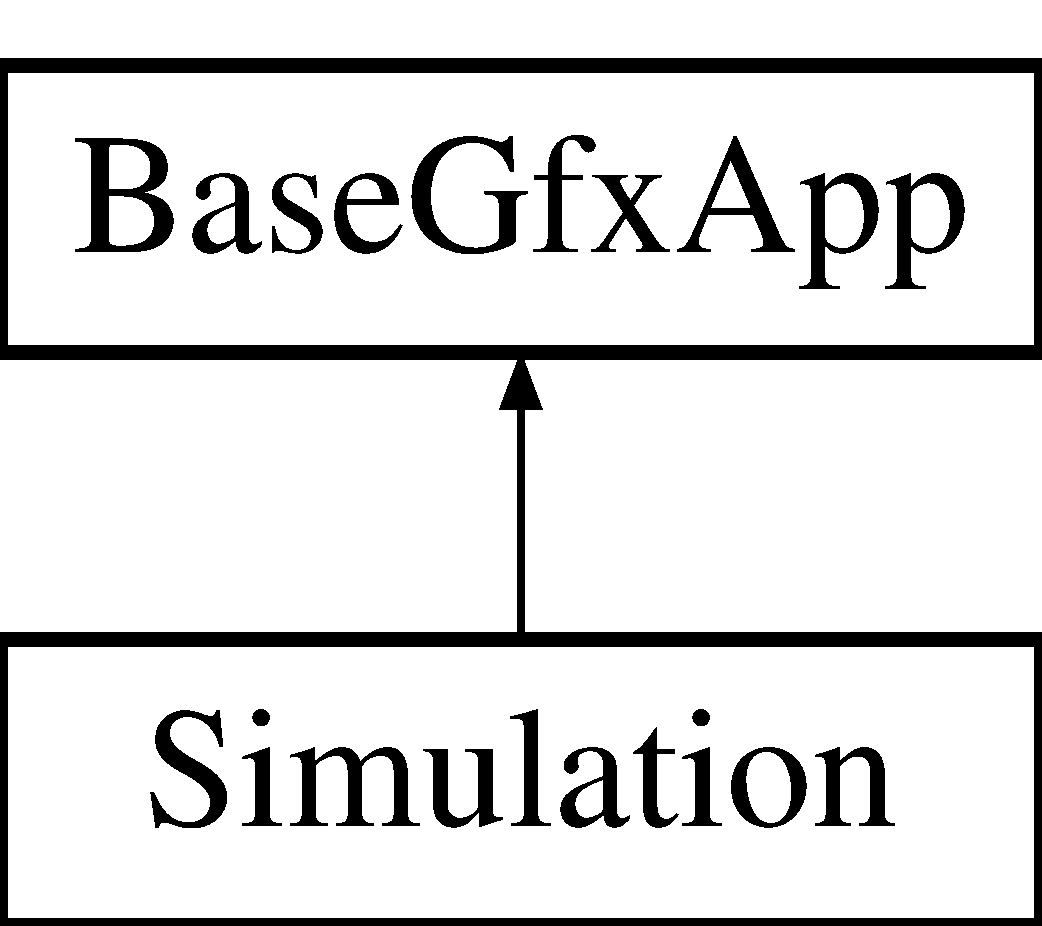
\includegraphics[height=2.000000cm]{classBaseGfxApp}
\end{center}
\end{figure}
\subsection*{Public Member Functions}
\begin{DoxyCompactItemize}
\item 
\hypertarget{classBaseGfxApp_a534a4b5293a35947fdae3805a103541d}{{\bfseries Base\-Gfx\-App} (int argc, char $\ast$argv\mbox{[}$\,$\mbox{]}, int width, int height, int x, int y, int glut\-Flags, bool create\-G\-L\-U\-I\-Win, int glui\-Win\-X, int glui\-Win\-Y)}\label{classBaseGfxApp_a534a4b5293a35947fdae3805a103541d}

\item 
\hypertarget{classBaseGfxApp_a4b3b1a475b7f2babaf1b477c34b15fb1}{void {\bfseries set\-Caption} (const std\-::string \&caption)}\label{classBaseGfxApp_a4b3b1a475b7f2babaf1b477c34b15fb1}

\item 
\hypertarget{classBaseGfxApp_acda031916c00d56c2dc901e2653e3083}{void {\bfseries run\-Main\-Loop} ()}\label{classBaseGfxApp_acda031916c00d56c2dc901e2653e3083}

\item 
\hypertarget{classBaseGfxApp_ac8de2d5a955582547af5619b771b4d6d}{virtual void {\bfseries display} ()}\label{classBaseGfxApp_ac8de2d5a955582547af5619b771b4d6d}

\item 
\hypertarget{classBaseGfxApp_a0956b82d7fa58b623c498aea7073dbba}{virtual void {\bfseries mouse\-Moved} (int x, int y)}\label{classBaseGfxApp_a0956b82d7fa58b623c498aea7073dbba}

\item 
\hypertarget{classBaseGfxApp_abb23f716dd6612b3a72938e41525d338}{virtual void {\bfseries mouse\-Dragged} (int x, int y)}\label{classBaseGfxApp_abb23f716dd6612b3a72938e41525d338}

\item 
\hypertarget{classBaseGfxApp_aaaccf5a5e923a9465441a5ee712424a8}{virtual void {\bfseries left\-Mouse\-Down} (int x, int y)}\label{classBaseGfxApp_aaaccf5a5e923a9465441a5ee712424a8}

\item 
\hypertarget{classBaseGfxApp_a0a2961a932b02b2f9d7d0bb408f6fb51}{virtual void {\bfseries left\-Mouse\-Up} (int x, int y)}\label{classBaseGfxApp_a0a2961a932b02b2f9d7d0bb408f6fb51}

\item 
\hypertarget{classBaseGfxApp_afa87e6a71220945e41f0424e540125d9}{virtual void {\bfseries right\-Mouse\-Down} (int x, int y)}\label{classBaseGfxApp_afa87e6a71220945e41f0424e540125d9}

\item 
\hypertarget{classBaseGfxApp_a812643d563522a993457dd565c33f8f6}{virtual void {\bfseries right\-Mouse\-Up} (int x, int y)}\label{classBaseGfxApp_a812643d563522a993457dd565c33f8f6}

\item 
\hypertarget{classBaseGfxApp_a2c98cae9bb5ad1fb1832a6d4812670f8}{virtual void {\bfseries middle\-Mouse\-Down} (int x, int y)}\label{classBaseGfxApp_a2c98cae9bb5ad1fb1832a6d4812670f8}

\item 
\hypertarget{classBaseGfxApp_a00fc05e8d9629b72302b5adf014bdb0c}{virtual void {\bfseries middle\-Mouse\-Up} (int x, int y)}\label{classBaseGfxApp_a00fc05e8d9629b72302b5adf014bdb0c}

\item 
\hypertarget{classBaseGfxApp_a6d91e0cb7a3d48cad33956efe7eb36ca}{virtual void {\bfseries keyboard} (unsigned char c, int x, int y)}\label{classBaseGfxApp_a6d91e0cb7a3d48cad33956efe7eb36ca}

\item 
\hypertarget{classBaseGfxApp_a345566e62c9e4ec3705ec4d1c4c75f1f}{virtual void {\bfseries keyboard\-Special} (int key, int x, int y)}\label{classBaseGfxApp_a345566e62c9e4ec3705ec4d1c4c75f1f}

\item 
\hypertarget{classBaseGfxApp_acc4a40ce11edd6b6660a19cb4802a2bf}{virtual void {\bfseries keyboard\-Up} (unsigned char c, int x, int y)}\label{classBaseGfxApp_acc4a40ce11edd6b6660a19cb4802a2bf}

\item 
\hypertarget{classBaseGfxApp_afd14b435ff93b1e7f461cb8bd1a6fd59}{virtual void {\bfseries keyboard\-Special\-Up} (int key, int x, int y)}\label{classBaseGfxApp_afd14b435ff93b1e7f461cb8bd1a6fd59}

\item 
\hypertarget{classBaseGfxApp_a5d8d5d778a8aecd7f5f8e9c87f4c3d20}{virtual void {\bfseries reshape} (int width, int height)}\label{classBaseGfxApp_a5d8d5d778a8aecd7f5f8e9c87f4c3d20}

\item 
\hypertarget{classBaseGfxApp_a2978a7c358794c67df73b66776b2cef3}{virtual void {\bfseries glui\-Control} (int control\-I\-D)}\label{classBaseGfxApp_a2978a7c358794c67df73b66776b2cef3}

\item 
\hypertarget{classBaseGfxApp_ace089a1a94fb6bb0bc17e1b7fa48e05d}{int {\bfseries width} () const }\label{classBaseGfxApp_ace089a1a94fb6bb0bc17e1b7fa48e05d}

\item 
\hypertarget{classBaseGfxApp_aa253dbe16a20c40e0a1bf8ff942ceea3}{int {\bfseries height} () const }\label{classBaseGfxApp_aa253dbe16a20c40e0a1bf8ff942ceea3}

\item 
\hypertarget{classBaseGfxApp_ae9779f948eff6f45beec08091e98a803}{int {\bfseries handle} ()}\label{classBaseGfxApp_ae9779f948eff6f45beec08091e98a803}

\item 
\hypertarget{classBaseGfxApp_ac721a0fedce80308c5c0e5695016e95d}{G\-L\-U\-I $\ast$ {\bfseries glui} ()}\label{classBaseGfxApp_ac721a0fedce80308c5c0e5695016e95d}

\end{DoxyCompactItemize}
\subsection*{Static Protected Member Functions}
\begin{DoxyCompactItemize}
\item 
\hypertarget{classBaseGfxApp_a5fe6a77d37044cbe28647ed3391bbb7a}{static void {\bfseries s\-\_\-reshape} (int width, int height)}\label{classBaseGfxApp_a5fe6a77d37044cbe28647ed3391bbb7a}

\item 
\hypertarget{classBaseGfxApp_a52edb2569227319feb68779844e7d857}{static void {\bfseries s\-\_\-keyboard} (unsigned char c, int x, int y)}\label{classBaseGfxApp_a52edb2569227319feb68779844e7d857}

\item 
\hypertarget{classBaseGfxApp_a1e8d90a4faab60300ddf2a4ea9b83115}{static void {\bfseries s\-\_\-keyboardspecial} (int key, int x, int y)}\label{classBaseGfxApp_a1e8d90a4faab60300ddf2a4ea9b83115}

\item 
\hypertarget{classBaseGfxApp_aa1ca205af9d6cee33949f2e6adf4c923}{static void {\bfseries s\-\_\-keyboardup} (unsigned char c, int x, int y)}\label{classBaseGfxApp_aa1ca205af9d6cee33949f2e6adf4c923}

\item 
\hypertarget{classBaseGfxApp_a0e4dfe006f3cc9126c1cc8ad32784f75}{static void {\bfseries s\-\_\-keyboardspecialup} (int key, int x, int y)}\label{classBaseGfxApp_a0e4dfe006f3cc9126c1cc8ad32784f75}

\item 
\hypertarget{classBaseGfxApp_a5e640f2394f7e038d0dd2b469d5c2e24}{static void {\bfseries s\-\_\-mousemotion} (int x, int y)}\label{classBaseGfxApp_a5e640f2394f7e038d0dd2b469d5c2e24}

\item 
\hypertarget{classBaseGfxApp_a22dd953bfb75add9fd0f8f2f8be535c5}{static void {\bfseries s\-\_\-mousebtn} (int b, int s, int x, int y)}\label{classBaseGfxApp_a22dd953bfb75add9fd0f8f2f8be535c5}

\item 
\hypertarget{classBaseGfxApp_a58415c6151a2a80e1fe2eaa9919a4dab}{static void {\bfseries s\-\_\-draw} ()}\label{classBaseGfxApp_a58415c6151a2a80e1fe2eaa9919a4dab}

\item 
\hypertarget{classBaseGfxApp_ad4a963321f1147d68369225ab0c7f32f}{static void {\bfseries s\-\_\-gluicallback} (int control\-I\-D)}\label{classBaseGfxApp_ad4a963321f1147d68369225ab0c7f32f}

\end{DoxyCompactItemize}
\subsection*{Protected Attributes}
\begin{DoxyCompactItemize}
\item 
int \hyperlink{classBaseGfxApp_ad8697d6fdd10e6f336c3a662016b4fa7}{m\-\_\-glut\-Window\-Handle}
\item 
\hypertarget{classBaseGfxApp_a6eb1673b80283727221da2242211af1d}{G\-L\-U\-I $\ast$ {\bfseries m\-\_\-glui}}\label{classBaseGfxApp_a6eb1673b80283727221da2242211af1d}

\item 
\hypertarget{classBaseGfxApp_a2e70a389224f8affe7c137f7e20dc8c1}{bool {\bfseries m\-\_\-drag}}\label{classBaseGfxApp_a2e70a389224f8affe7c137f7e20dc8c1}

\item 
\hypertarget{classBaseGfxApp_a7e5ef1c8f25fe081b4a1fd4ce6a96e07}{int {\bfseries m\-\_\-width}}\label{classBaseGfxApp_a7e5ef1c8f25fe081b4a1fd4ce6a96e07}

\item 
\hypertarget{classBaseGfxApp_ac078e4fc20b5c2fe0c744966b850b412}{int {\bfseries m\-\_\-height}}\label{classBaseGfxApp_ac078e4fc20b5c2fe0c744966b850b412}

\end{DoxyCompactItemize}
\subsection*{Static Protected Attributes}
\begin{DoxyCompactItemize}
\item 
static \hyperlink{classBaseGfxApp}{Base\-Gfx\-App} $\ast$ \hyperlink{classBaseGfxApp_a65ba89b98af31e2649a0546631931000}{s\-\_\-current\-App} = N\-U\-L\-L
\item 
static bool \hyperlink{classBaseGfxApp_afa4690383ea27713016ef75b9fb1e42f}{s\-\_\-glut\-Initialized} = false
\end{DoxyCompactItemize}


\subsection{Detailed Description}
based \hyperlink{classBaseGfxApp}{Base\-Gfx\-App} 

\subsection{Member Data Documentation}
\hypertarget{classBaseGfxApp_ad8697d6fdd10e6f336c3a662016b4fa7}{\index{Base\-Gfx\-App@{Base\-Gfx\-App}!m\-\_\-glut\-Window\-Handle@{m\-\_\-glut\-Window\-Handle}}
\index{m\-\_\-glut\-Window\-Handle@{m\-\_\-glut\-Window\-Handle}!BaseGfxApp@{Base\-Gfx\-App}}
\subsubsection[{m\-\_\-glut\-Window\-Handle}]{\setlength{\rightskip}{0pt plus 5cm}int Base\-Gfx\-App\-::m\-\_\-glut\-Window\-Handle\hspace{0.3cm}{\ttfamily [protected]}}}\label{classBaseGfxApp_ad8697d6fdd10e6f336c3a662016b4fa7}
Underlying glut window handle \hypertarget{classBaseGfxApp_a65ba89b98af31e2649a0546631931000}{\index{Base\-Gfx\-App@{Base\-Gfx\-App}!s\-\_\-current\-App@{s\-\_\-current\-App}}
\index{s\-\_\-current\-App@{s\-\_\-current\-App}!BaseGfxApp@{Base\-Gfx\-App}}
\subsubsection[{s\-\_\-current\-App}]{\setlength{\rightskip}{0pt plus 5cm}{\bf Base\-Gfx\-App} $\ast$ Base\-Gfx\-App\-::s\-\_\-current\-App = N\-U\-L\-L\hspace{0.3cm}{\ttfamily [static]}, {\ttfamily [protected]}}}\label{classBaseGfxApp_a65ba89b98af31e2649a0546631931000}
G\-L\-U\-T and G\-L\-U\-I event callbacks are sent to the current window/app. Right now, there is only one window anyway (not counting the G\-L\-U\-I U\-I window.. in the future could be extended to support more windows. In any case, some structure like this is always needed when using glut with C++, since the glut callbacks must be either global or static functions. \hypertarget{classBaseGfxApp_afa4690383ea27713016ef75b9fb1e42f}{\index{Base\-Gfx\-App@{Base\-Gfx\-App}!s\-\_\-glut\-Initialized@{s\-\_\-glut\-Initialized}}
\index{s\-\_\-glut\-Initialized@{s\-\_\-glut\-Initialized}!BaseGfxApp@{Base\-Gfx\-App}}
\subsubsection[{s\-\_\-glut\-Initialized}]{\setlength{\rightskip}{0pt plus 5cm}bool Base\-Gfx\-App\-::s\-\_\-glut\-Initialized = false\hspace{0.3cm}{\ttfamily [static]}, {\ttfamily [protected]}}}\label{classBaseGfxApp_afa4690383ea27713016ef75b9fb1e42f}
Has glut\-Init been called? (only allowed once per program) 

The documentation for this class was generated from the following files\-:\begin{DoxyCompactItemize}
\item 
\hyperlink{BaseGfxApp_8h}{Base\-Gfx\-App.\-h}\item 
\hyperlink{BaseGfxApp_8cpp}{Base\-Gfx\-App.\-cpp}\end{DoxyCompactItemize}

\hypertarget{classCircularObstacle}{\section{Circular\-Obstacle Class Reference}
\label{classCircularObstacle}\index{Circular\-Obstacle@{Circular\-Obstacle}}
}


obstacle with circul  




{\ttfamily \#include $<$Obstacle.\-h$>$}

Inheritance diagram for Circular\-Obstacle\-:\begin{figure}[H]
\begin{center}
\leavevmode
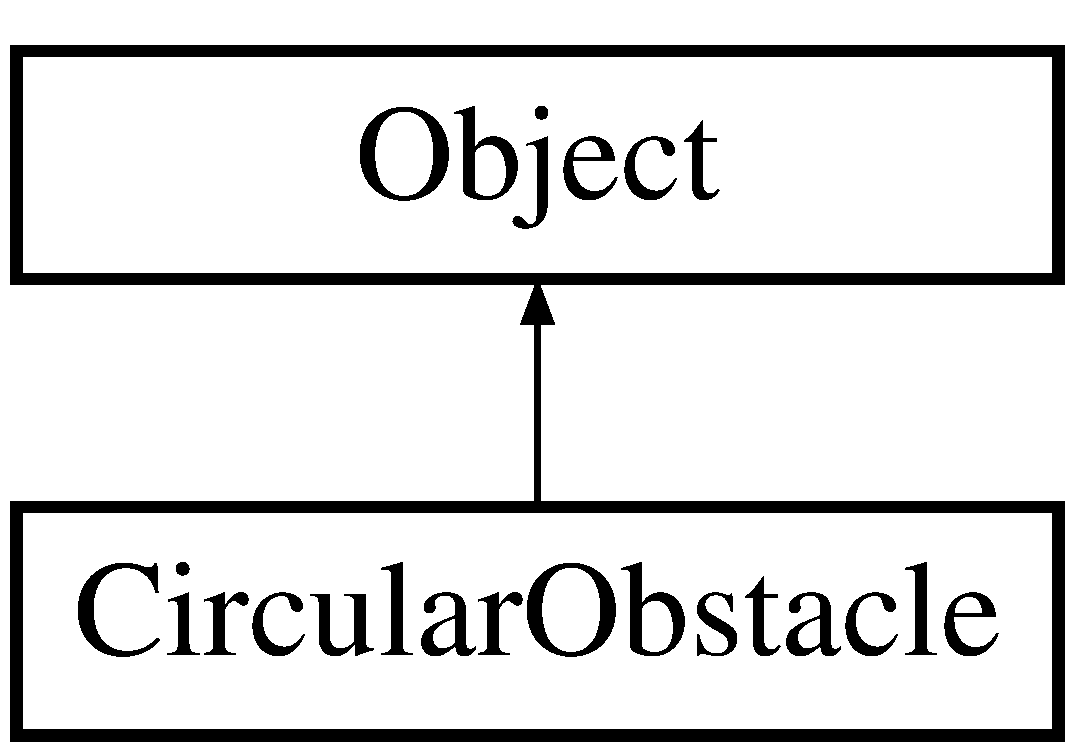
\includegraphics[height=2.000000cm]{classCircularObstacle}
\end{center}
\end{figure}
\subsection*{Public Member Functions}
\begin{DoxyCompactItemize}
\item 
\hyperlink{classCircularObstacle_ad219c09015b786e7e2730b10f9860c26}{Circular\-Obstacle} ()
\begin{DoxyCompactList}\small\item\em class \hyperlink{classCircularObstacle}{Circular\-Obstacle} default constuctor \end{DoxyCompactList}\item 
\hyperlink{classCircularObstacle_a816a0b717d09898e52204298a05b38ad}{Circular\-Obstacle} (const \hyperlink{structGLPosition}{G\-L\-Position} \&pos, const G\-Lint r)
\begin{DoxyCompactList}\small\item\em class \hyperlink{classCircularObstacle}{Circular\-Obstacle} constuctor \end{DoxyCompactList}\item 
\hypertarget{classCircularObstacle_ae1cfdaf0e619db408370cea8472b6a9b}{virtual void \hyperlink{classCircularObstacle_ae1cfdaf0e619db408370cea8472b6a9b}{move} (const time\-\_\-t elapsed\-Time)}\label{classCircularObstacle_ae1cfdaf0e619db408370cea8472b6a9b}

\begin{DoxyCompactList}\small\item\em go on a pleasure trip this obstacle \end{DoxyCompactList}\item 
\hypertarget{classCircularObstacle_a71b41d366d8507a233ffd2f1fc8f3587}{virtual void \hyperlink{classCircularObstacle_a71b41d366d8507a233ffd2f1fc8f3587}{render} (const \hyperlink{Common_8h_a5113b6588451c418d38d8b3681eb6040}{gl\-Color\-Vec} \&c)}\label{classCircularObstacle_a71b41d366d8507a233ffd2f1fc8f3587}

\begin{DoxyCompactList}\small\item\em set color use {\ttfamily } \end{DoxyCompactList}\item 
\hypertarget{classCircularObstacle_ae1cb1117a74485ddbd7ed3c9e846cfa1}{virtual bool \hyperlink{classCircularObstacle_ae1cb1117a74485ddbd7ed3c9e846cfa1}{detect\-Collision} ()}\label{classCircularObstacle_ae1cb1117a74485ddbd7ed3c9e846cfa1}

\begin{DoxyCompactList}\small\item\em check if collision with any other object \end{DoxyCompactList}\item 
\hypertarget{classCircularObstacle_a6a795a94b3df599203bd94f7098a0c65}{virtual void \hyperlink{classCircularObstacle_a6a795a94b3df599203bd94f7098a0c65}{rotate} (const G\-Lint \&deg)}\label{classCircularObstacle_a6a795a94b3df599203bd94f7098a0c65}

\begin{DoxyCompactList}\small\item\em ratote  degrees \end{DoxyCompactList}\item 
\hypertarget{classCircularObstacle_a888250b42230e2b6f5711428d3f20854}{virtual void \hyperlink{classCircularObstacle_a888250b42230e2b6f5711428d3f20854}{update\-Position} (const \hyperlink{structGLPosition}{G\-L\-Position} \&new\-Pos)}\label{classCircularObstacle_a888250b42230e2b6f5711428d3f20854}

\begin{DoxyCompactList}\small\item\em update position with  \end{DoxyCompactList}\item 
\hypertarget{classCircularObstacle_a4389dbe384efd2055adfbf2bfd8c8683}{G\-Lint \hyperlink{classCircularObstacle_a4389dbe384efd2055adfbf2bfd8c8683}{get\-Radius} () const }\label{classCircularObstacle_a4389dbe384efd2055adfbf2bfd8c8683}

\begin{DoxyCompactList}\small\item\em get the radius \end{DoxyCompactList}\end{DoxyCompactItemize}
\subsection*{Public Attributes}
\begin{DoxyCompactItemize}
\item 
\hypertarget{classCircularObstacle_adb4bc2ee2ab0a7ee03571663976bd2e1}{G\-Lint {\bfseries radius}}\label{classCircularObstacle_adb4bc2ee2ab0a7ee03571663976bd2e1}

\item 
\hypertarget{classCircularObstacle_adaa9bb8650d122ec2891a81d22fcb8fa}{G\-Lint {\bfseries speed}}\label{classCircularObstacle_adaa9bb8650d122ec2891a81d22fcb8fa}

\item 
\hypertarget{classCircularObstacle_a6bd3428e3a01544f7e29fe4ec2df95ca}{G\-Lint {\bfseries direction}}\label{classCircularObstacle_a6bd3428e3a01544f7e29fe4ec2df95ca}

\item 
\hypertarget{classCircularObstacle_aee1b031760bcaafed15496debe10197b}{bool {\bfseries motionless}}\label{classCircularObstacle_aee1b031760bcaafed15496debe10197b}

\item 
\hypertarget{classCircularObstacle_afeafb626ba908916fec5272442c0dbf1}{\hyperlink{Common_8h_a5113b6588451c418d38d8b3681eb6040}{gl\-Color\-Vec} {\bfseries color}}\label{classCircularObstacle_afeafb626ba908916fec5272442c0dbf1}

\end{DoxyCompactItemize}
\subsection*{Protected Member Functions}
\begin{DoxyCompactItemize}
\item 
virtual void \hyperlink{classCircularObstacle_a9e129c320c72141afebbfa5bc299a15e}{draw} ()
\begin{DoxyCompactList}\small\item\em draw a circle obstacle by defined color \end{DoxyCompactList}\end{DoxyCompactItemize}
\subsection*{Additional Inherited Members}


\subsection{Detailed Description}
obstacle with circul 

\subsection{Constructor \& Destructor Documentation}
\hypertarget{classCircularObstacle_ad219c09015b786e7e2730b10f9860c26}{\index{Circular\-Obstacle@{Circular\-Obstacle}!Circular\-Obstacle@{Circular\-Obstacle}}
\index{Circular\-Obstacle@{Circular\-Obstacle}!CircularObstacle@{Circular\-Obstacle}}
\subsubsection[{Circular\-Obstacle}]{\setlength{\rightskip}{0pt plus 5cm}Circular\-Obstacle\-::\-Circular\-Obstacle (
\begin{DoxyParamCaption}
{}
\end{DoxyParamCaption}
)}}\label{classCircularObstacle_ad219c09015b786e7e2730b10f9860c26}


class \hyperlink{classCircularObstacle}{Circular\-Obstacle} default constuctor 

\begin{DoxyAuthor}{Author}
Jiajun Ni 
\end{DoxyAuthor}
\hypertarget{classCircularObstacle_a816a0b717d09898e52204298a05b38ad}{\index{Circular\-Obstacle@{Circular\-Obstacle}!Circular\-Obstacle@{Circular\-Obstacle}}
\index{Circular\-Obstacle@{Circular\-Obstacle}!CircularObstacle@{Circular\-Obstacle}}
\subsubsection[{Circular\-Obstacle}]{\setlength{\rightskip}{0pt plus 5cm}Circular\-Obstacle\-::\-Circular\-Obstacle (
\begin{DoxyParamCaption}
\item[{const {\bf G\-L\-Position} \&}]{pos, }
\item[{const G\-Lint}]{r}
\end{DoxyParamCaption}
)}}\label{classCircularObstacle_a816a0b717d09898e52204298a05b38ad}


class \hyperlink{classCircularObstacle}{Circular\-Obstacle} constuctor 


\begin{DoxyCode}
  rand generate direction,set speed to fixed 2 pixels
  and use user\textcolor{stringliteral}{'s setting}
\textcolor{stringliteral}{  /}
\textcolor{stringliteral}{srand(time(NULL));}
\textcolor{stringliteral}{direction = rand() % 360;}
\textcolor{stringliteral}{}
\textcolor{stringliteral}{speed = 2;}
\textcolor{stringliteral}{}
\textcolor{stringliteral}{radius = r;}
\textcolor{stringliteral}{position = pos;}
\end{DoxyCode}
 

\subsection{Member Function Documentation}
\hypertarget{classCircularObstacle_a9e129c320c72141afebbfa5bc299a15e}{\index{Circular\-Obstacle@{Circular\-Obstacle}!draw@{draw}}
\index{draw@{draw}!CircularObstacle@{Circular\-Obstacle}}
\subsubsection[{draw}]{\setlength{\rightskip}{0pt plus 5cm}void Circular\-Obstacle\-::draw (
\begin{DoxyParamCaption}
{}
\end{DoxyParamCaption}
)\hspace{0.3cm}{\ttfamily [protected]}, {\ttfamily [virtual]}}}\label{classCircularObstacle_a9e129c320c72141afebbfa5bc299a15e}


draw a circle obstacle by defined color 


\begin{DoxyCode}
 circle represent obstacles. */
\textcolor{keywordflow}{for} (\textcolor{keywordtype}{int} i = 0; i <= sections; i++)
\{
    glVertex2f(position.posX + radius * cos(i * TWOPI / sections), position.posY + radius * sin(i * TWOPI /
       sections));
\}

glEnd();
\end{DoxyCode}
 

Implements \hyperlink{classObject_a59f4160d4d035e85ebdd706acdcd60f9}{Object}.



The documentation for this class was generated from the following files\-:\begin{DoxyCompactItemize}
\item 
\hyperlink{Obstacle_8h}{Obstacle.\-h}\item 
Obstacle.\-cpp\end{DoxyCompactItemize}

\hypertarget{classCommonTests}{\section{Common\-Tests Class Reference}
\label{classCommonTests}\index{Common\-Tests@{Common\-Tests}}
}


test function for G\-Lposition struct, object overlapping and detect\-Wall  




{\ttfamily \#include $<$Common\-Test.\-h$>$}

Inheritance diagram for Common\-Tests\-:\begin{figure}[H]
\begin{center}
\leavevmode
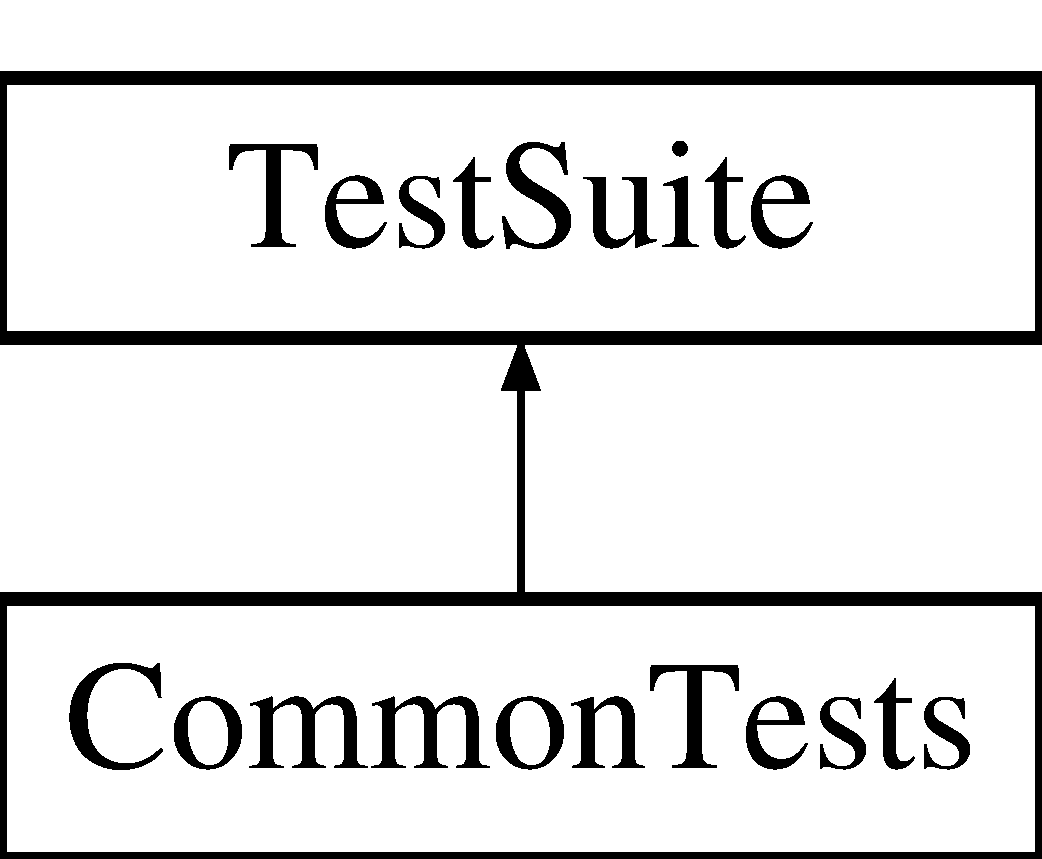
\includegraphics[height=2.000000cm]{classCommonTests}
\end{center}
\end{figure}
\subsection*{Public Member Functions}
\begin{DoxyCompactItemize}
\item 
\hypertarget{classCommonTests_a7b4e7469ca8ac289b9dc4ec52a454e0b}{void {\bfseries Test\-\_\-\-G\-L\-Position\-E\-Q} (void)}\label{classCommonTests_a7b4e7469ca8ac289b9dc4ec52a454e0b}

\item 
\hypertarget{classCommonTests_ab3fd4ebe7420eb8d9aa442c3754ad024}{void {\bfseries Test\-\_\-\-Object\-\_\-detect\-Overlapping} ()}\label{classCommonTests_ab3fd4ebe7420eb8d9aa442c3754ad024}

\item 
\hypertarget{classCommonTests_ac02de5286f53e2ab33de69298db6e6ea}{void {\bfseries test\-\_\-detect\-Wall} (void)}\label{classCommonTests_ac02de5286f53e2ab33de69298db6e6ea}

\end{DoxyCompactItemize}


\subsection{Detailed Description}
test function for G\-Lposition struct, object overlapping and detect\-Wall 

The documentation for this class was generated from the following file\-:\begin{DoxyCompactItemize}
\item 
\hyperlink{CommonTest_8h}{Common\-Test.\-h}\end{DoxyCompactItemize}

\hypertarget{classEnvironmentClass}{\section{Environment\-Class Class Reference}
\label{classEnvironmentClass}\index{Environment\-Class@{Environment\-Class}}
}


Class to contain physical objects, sizes/position of all objects and contains info on where the borders are in the window.  




{\ttfamily \#include $<$Environment\-Class.\-h$>$}

\subsection*{Public Types}
\begin{DoxyCompactItemize}
\item 
\hypertarget{classEnvironmentClass_a563d291dc565587df66e61b8bca1cd91}{typedef std\-::vector$<$ std\-::pair\\*
$<$ std\-::pair$<$ double, double $>$\\*
, double $>$ $>$ {\bfseries Offset\-Triangle}}\label{classEnvironmentClass_a563d291dc565587df66e61b8bca1cd91}

\end{DoxyCompactItemize}
\subsection*{Public Member Functions}
\begin{DoxyCompactItemize}
\item 
void \hyperlink{classEnvironmentClass_a2ea61074efd8e3f099e2876a101c219f}{update} ()
\begin{DoxyCompactList}\small\item\em update simulating scene, such as robot's angle, object's posiion, etc \end{DoxyCompactList}\end{DoxyCompactItemize}
\subsection*{Static Public Member Functions}
\begin{DoxyCompactItemize}
\item 
static void \hyperlink{classEnvironmentClass_a3af1904397a45c74acbc0c8246c0317d}{init} (const G\-Lint \&width, const G\-Lint \&height)
\begin{DoxyCompactList}\small\item\em init the scene, create both robots and obstacles, place them randomly, \end{DoxyCompactList}\item 
static bool \hyperlink{classEnvironmentClass_a52f4e00b563733c2019204d16de139b9}{sense\-Touch} (\hyperlink{classObject}{Object} $\ast$p\-Object)
\begin{DoxyCompactList}\small\item\em the senser for {\itshape Touch}  -\/ the detect object  -\/ the flag to indicate if the  is deleted? \end{DoxyCompactList}\item 
static double \hyperlink{classEnvironmentClass_a5b501f7123ca5ba7fd711a44a3d0141e}{sense\-Homing} (const \hyperlink{classRobotClass}{Robot\-Class} $\ast$p\-Robot, const \hyperlink{classObject}{Object} $\ast$p\-Target)
\begin{DoxyCompactList}\small\item\em the senser for {\itshape Homing}, it base on the rectangular coordinate system \end{DoxyCompactList}\end{DoxyCompactItemize}
\subsection*{Static Public Attributes}
\begin{DoxyCompactItemize}
\item 
static std\-::vector\\*
$<$ \hyperlink{classCircularObstacle}{Circular\-Obstacle} $\ast$ $>$ \hyperlink{classEnvironmentClass_a738593c1c3ed257bea8f99f663f59d85}{vec\-Obstacle}
\item 
\hypertarget{classEnvironmentClass_aad109138f5c22257a6d2827ac4c5f70c}{static std\-::vector$<$ \hyperlink{classRobotClass}{Robot\-Class} $\ast$ $>$ {\bfseries vec\-Robot}}\label{classEnvironmentClass_aad109138f5c22257a6d2827ac4c5f70c}

\item 
\hypertarget{classEnvironmentClass_af1e7176105de214ec957d3f7452992a4}{static int {\bfseries win\-Width} = 0}\label{classEnvironmentClass_af1e7176105de214ec957d3f7452992a4}

\item 
\hypertarget{classEnvironmentClass_a59a6025ef7ffc092995111b53a316767}{static int {\bfseries win\-Height} = 0}\label{classEnvironmentClass_a59a6025ef7ffc092995111b53a316767}

\item 
\hypertarget{classEnvironmentClass_ad5de7d6824468cb6ea5ba09b9f10c114}{static \hyperlink{Common_8h_a5113b6588451c418d38d8b3681eb6040}{gl\-Color\-Vec} {\bfseries collided\-Color} = \hyperlink{Common_8h_a5113b6588451c418d38d8b3681eb6040}{gl\-Color\-Vec}(101, 106, 100)}\label{classEnvironmentClass_ad5de7d6824468cb6ea5ba09b9f10c114}

\end{DoxyCompactItemize}
\subsection*{Static Protected Member Functions}
\begin{DoxyCompactItemize}
\item 
static \hyperlink{structGLPosition}{G\-L\-Position} \hyperlink{classEnvironmentClass_a330bbca10dbd5743714d7e722748ae47}{generate\-Rand\-Position} (const G\-Lint \&width, const G\-Lint \&height, const G\-Lint \&bounding\-Width, const G\-Lint \&bounding\-Height)
\begin{DoxyCompactList}\small\item\em generate a rand position for any object, base on its bounding rectangle \end{DoxyCompactList}\item 
static double \hyperlink{classEnvironmentClass_a3fa1b87f8ae74bf1cefda9862e1bdfca}{distance} (const \hyperlink{structGLPosition}{G\-L\-Position} \&pos1, const \hyperlink{structGLPosition}{G\-L\-Position} \&pos2)
\begin{DoxyCompactList}\small\item\em calculate the distance between  and   -\/ the start posion  -\/ the end posion \end{DoxyCompactList}\end{DoxyCompactItemize}
\subsection*{Friends}
\begin{DoxyCompactItemize}
\item 
\hypertarget{classEnvironmentClass_a5b6e810512e47f0467ef729ad744bc3f}{class \hyperlink{classEnvironmentClass_a5b6e810512e47f0467ef729ad744bc3f}{Environment\-Class\-Tests}}\label{classEnvironmentClass_a5b6e810512e47f0467ef729ad744bc3f}

\begin{DoxyCompactList}\small\item\em Friend for class test. \end{DoxyCompactList}\end{DoxyCompactItemize}


\subsection{Detailed Description}
Class to contain physical objects, sizes/position of all objects and contains info on where the borders are in the window. 

\subsection{Member Function Documentation}
\hypertarget{classEnvironmentClass_a3fa1b87f8ae74bf1cefda9862e1bdfca}{\index{Environment\-Class@{Environment\-Class}!distance@{distance}}
\index{distance@{distance}!EnvironmentClass@{Environment\-Class}}
\subsubsection[{distance}]{\setlength{\rightskip}{0pt plus 5cm}double Environment\-Class\-::distance (
\begin{DoxyParamCaption}
\item[{const {\bf G\-L\-Position} \&}]{pos1, }
\item[{const {\bf G\-L\-Position} \&}]{pos2}
\end{DoxyParamCaption}
)\hspace{0.3cm}{\ttfamily [static]}, {\ttfamily [protected]}}}\label{classEnvironmentClass_a3fa1b87f8ae74bf1cefda9862e1bdfca}


calculate the distance between  and   -\/ the start posion  -\/ the end posion 

calculate the distance between  and 

\begin{DoxyAuthor}{Author}
Jiajun Ni 
\end{DoxyAuthor}
\begin{DoxyReturn}{Returns}
-\/ the distance between  and  
\end{DoxyReturn}

\begin{DoxyCode}
   \textcolor{keywordflow}{if} the @pos1 and @pos2 form a right angled triangle, use the pythagorean theorem to calculate
   the \hyperlink{classEnvironmentClass_a3fa1b87f8ae74bf1cefda9862e1bdfca}{distance}. otherwise, calculate it directly.
  /
\textcolor{keywordflow}{if} (pos1.posX != pos2.posX && pos1.posY != pos2.posY)
\{
    GLint a = abs(pos1.posX - pos2.posX);
    GLint b = abs(pos1.posY - pos2.posY);
    
    \hyperlink{classEnvironmentClass_a3fa1b87f8ae74bf1cefda9862e1bdfca}{distance} = sqrt(pow(a, 2) + pow(b, 2));
\}
\textcolor{keywordflow}{else}
\{
    \textcolor{keywordflow}{if} (pos1.posX == pos2.posX)
    \{
        \hyperlink{classEnvironmentClass_a3fa1b87f8ae74bf1cefda9862e1bdfca}{distance} = abs(pos1.posY - pos2.posY);
    \}
    
    \textcolor{keywordflow}{if} (pos1.posY == pos2.posY)
    \{
        \hyperlink{classEnvironmentClass_a3fa1b87f8ae74bf1cefda9862e1bdfca}{distance} = abs(pos1.posX - pos2.posX);
    \}
\}
\end{DoxyCode}
\hypertarget{classEnvironmentClass_a330bbca10dbd5743714d7e722748ae47}{\index{Environment\-Class@{Environment\-Class}!generate\-Rand\-Position@{generate\-Rand\-Position}}
\index{generate\-Rand\-Position@{generate\-Rand\-Position}!EnvironmentClass@{Environment\-Class}}
\subsubsection[{generate\-Rand\-Position}]{\setlength{\rightskip}{0pt plus 5cm}{\bf G\-L\-Position} Environment\-Class\-::generate\-Rand\-Position (
\begin{DoxyParamCaption}
\item[{const G\-Lint \&}]{width, }
\item[{const G\-Lint \&}]{height, }
\item[{const G\-Lint \&}]{bounding\-Width, }
\item[{const G\-Lint \&}]{bounding\-Height}
\end{DoxyParamCaption}
)\hspace{0.3cm}{\ttfamily [static]}, {\ttfamily [protected]}}}\label{classEnvironmentClass_a330bbca10dbd5743714d7e722748ae47}


generate a rand position for any object, base on its bounding rectangle 

generate a rand position for any object, base on its bounding rectangle

\begin{DoxyAuthor}{Author}
Jiajun Ni  -\/ G\-U\-I window width  -\/ G\-U\-I window height  -\/ the bounding rectangle with  -\/ the bounding rectangle height
\end{DoxyAuthor}
if successed, \begin{DoxyReturn}{Returns}
the generated posion, otherwise, 

(0, 0, 0) 
\end{DoxyReturn}
\begin{DoxyRefDesc}{Todo}
\item[\hyperlink{todo__todo000004}{Todo}]the poston must in the window \end{DoxyRefDesc}



\begin{DoxyCode}
   check \textcolor{keywordflow}{if} the current \textcolor{keywordtype}{object} over lapped any robot
   check \textcolor{keywordflow}{if} the robot completely contain \textcolor{keyword}{this} \textcolor{keywordtype}{object}
   check \textcolor{keywordflow}{if} the robot over lapped the \textcolor{keywordtype}{object}
  /  
\textcolor{keywordflow}{for} (std::size\_t i = 0; i < vecRobot.size(); i++)
\{
    \textcolor{keywordflow}{if} (\hyperlink{classEnvironmentClass_a3fa1b87f8ae74bf1cefda9862e1bdfca}{distance}(\hyperlink{structGLPosition}{GLPosition}(posX, posY, 0), vecRobot[i]->position) < vecRobot[i]->
      getRadius() + std::max(boundingWidth,
            boundingHeight))
    \{
        overlapped = \textcolor{keyword}{true};
        \textcolor{keywordflow}{break};
    \}
    
    \textcolor{keywordflow}{if} (vecRobot[i]->detectOverlapping(leftTop, rightBottom, vecRobot[i]->getRadius()))
    \{
        overlapped = \textcolor{keyword}{true};
        \textcolor{keywordflow}{break};
    \}
\}
\end{DoxyCode}



\begin{DoxyCode}
    check \textcolor{keywordflow}{if} the obstacle completely contain \textcolor{keyword}{this} \textcolor{keywordtype}{object}
    check \textcolor{keywordflow}{if} the robot over lapped the robot
    \textcolor{keywordflow}{if} the position is over lapped, it should be ignored
   / 
\textcolor{keywordflow}{for} (std::size\_t i = 0; i < \hyperlink{classEnvironmentClass_a738593c1c3ed257bea8f99f663f59d85}{vecObstacle}.size(); i++)
\{
    \textcolor{keywordflow}{if} (\hyperlink{classEnvironmentClass_a3fa1b87f8ae74bf1cefda9862e1bdfca}{distance}(\hyperlink{structGLPosition}{GLPosition}(posX, posY, 0), \hyperlink{classEnvironmentClass_a738593c1c3ed257bea8f99f663f59d85}{vecObstacle}[i]->position) < 
      \hyperlink{classEnvironmentClass_a738593c1c3ed257bea8f99f663f59d85}{vecObstacle}[i]->getRadius() + std::max(boundingWidth,
            boundingHeight))
    \{
        overlapped = \textcolor{keyword}{true};
        \textcolor{keywordflow}{break};
    \}
    
    \textcolor{keywordflow}{if} (\hyperlink{classEnvironmentClass_a738593c1c3ed257bea8f99f663f59d85}{vecObstacle}[i]->detectOverlapping(leftTop, rightBottom, 
      \hyperlink{classEnvironmentClass_a738593c1c3ed257bea8f99f663f59d85}{vecObstacle}[i]->getRadius()))
    \{
        overlapped = \textcolor{keyword}{true};
        \textcolor{keywordflow}{break};
    \}
\}
\end{DoxyCode}
\hypertarget{classEnvironmentClass_a3af1904397a45c74acbc0c8246c0317d}{\index{Environment\-Class@{Environment\-Class}!init@{init}}
\index{init@{init}!EnvironmentClass@{Environment\-Class}}
\subsubsection[{init}]{\setlength{\rightskip}{0pt plus 5cm}void Environment\-Class\-::init (
\begin{DoxyParamCaption}
\item[{const G\-Lint \&}]{width, }
\item[{const G\-Lint \&}]{height}
\end{DoxyParamCaption}
)\hspace{0.3cm}{\ttfamily [static]}}}\label{classEnvironmentClass_a3af1904397a45c74acbc0c8246c0317d}


init the scene, create both robots and obstacles, place them randomly, 

init the scene, create both robots and obstacles, place them randomly, and match the robot and its target.

\begin{DoxyAuthor}{Author}
Jiajun Ni  G\-U\-I window width  G\-U\-I window height no return value 
\end{DoxyAuthor}

\begin{DoxyCode}
   initialize robot objects
   set robot radius to 16 pixels,
   generate a rand posion \textcolor{keywordflow}{for} the robot.
   Set robot \textcolor{keywordtype}{id} and type with speed:8px.
   appointed target obstacle,set \textcolor{keywordflow}{default} color,different direction line color \textcolor{keywordflow}{for} different robot,
   add the robot instance to the vector
  / 
\textcolor{keywordflow}{for} (\textcolor{keywordtype}{int} i = 0; i < 2; i++)
\{
    GLint robotRadius = 16;
    \hyperlink{structGLPosition}{GLPosition} robotPos = \hyperlink{classEnvironmentClass_a330bbca10dbd5743714d7e722748ae47}{generateRandPosition}(width, height, robotRadius, 
      robotRadius);
    \hyperlink{classRobotClass}{RobotClass} *pRobot = \textcolor{keyword}{new}(std::nothrow) \hyperlink{classRobotClass}{RobotClass}(robotPos, robotRadius, 0);
    
    \textcolor{keywordflow}{if} (NULL == pRobot)
        \textcolor{keywordflow}{continue};
    pRobot->id = 1000 + i;
    pRobot->type = Object::eRobot;
    pRobot->\hyperlink{classRobotClass_ada07c364411e6d4c3efd6c5f5e4e6275}{setSpeed}(8);
    
    pRobot->setTarget(i * 2 + 1010);
    pRobot->\hyperlink{classRobotClass_af2069bec3bb391b05676e154527674fa}{render}(\hyperlink{Common_8h_a5113b6588451c418d38d8b3681eb6040}{glColorVec}(0.0f, 80.0f, 100.0f));
     
    \textcolor{keywordflow}{if} (i % 2)
        pRobot->setDirectionColor(\hyperlink{Common_8h_a5113b6588451c418d38d8b3681eb6040}{glColorVec}(100, 0, 0));
    \textcolor{keywordflow}{else}
        pRobot->setDirectionColor(\hyperlink{Common_8h_a5113b6588451c418d38d8b3681eb6040}{glColorVec}(200, 0, 100));
         
    vecRobot.push\_back(pRobot);
\}
\end{DoxyCode}


\begin{DoxyRefDesc}{Todo}
\item[\hyperlink{todo__todo000001}{Todo}]must create 2 robots \end{DoxyRefDesc}



\begin{DoxyCode}
   initialize obstacle objects,
   rand generater radius \textcolor{keywordflow}{for} obstacle, it between [16, 48) pixels
   generate a rand posion \textcolor{keywordflow}{for} the obstacle and \textcolor{keyword}{new} circular obstacle instance
   set obstacle \textcolor{keywordtype}{id},type, \textcolor{keywordflow}{default} color, 
   \textcolor{keywordflow}{if} \textcolor{keyword}{this} obstacle is appointed to a robot, use the robot\textcolor{stringliteral}{'s direction line color to draw it}
\textcolor{stringliteral}{   add to the obstacle vector}
\textcolor{stringliteral}{  / }
\textcolor{stringliteral}{for (int i = 0; i < 8; i++)}
\textcolor{stringliteral}{\{}
\textcolor{stringliteral}{    GLint obsRadius = rand() % 32 + 50; }
\textcolor{stringliteral}{    GLPosition obsPos = generateRandPosition(width, height, obsRadius, obsRadius);}
\textcolor{stringliteral}{    CircularObstacle *pCircObs = new(std::nothrow) CircularObstacle(obsPos, obsRadius);}
\textcolor{stringliteral}{    }
\textcolor{stringliteral}{    if (NULL == pCircObs)}
\textcolor{stringliteral}{        continue;}
\textcolor{stringliteral}{    }
\textcolor{stringliteral}{    pCircObs->id = 1010 + i;}
\textcolor{stringliteral}{   }
\textcolor{stringliteral}{    pCircObs->type = Object::eCircular;}
\textcolor{stringliteral}{    }
\textcolor{stringliteral}{    pCircObs->render(glColorVec(0, 100, 0));}
\textcolor{stringliteral}{    }
\textcolor{stringliteral}{    for (std::size\_t j = 0; j < vecRobot.size(); j++)}
\textcolor{stringliteral}{    \{}
\textcolor{stringliteral}{        if (vecRobot[j]->target() != pCircObs->id)}
\textcolor{stringliteral}{            continue;}
\textcolor{stringliteral}{            }
\textcolor{stringliteral}{        pCircObs->motionless = false;}
\textcolor{stringliteral}{        pCircObs->render(vecRobot[j]->directionColor());}
\textcolor{stringliteral}{    \}}
\textcolor{stringliteral}{    vecObstacle.push\_back(pCircObs);}
\textcolor{stringliteral}{\}}
\end{DoxyCode}


\begin{DoxyRefDesc}{Todo}
\item[\hyperlink{todo__todo000002}{Todo}]must create 6 circular obstacle \end{DoxyRefDesc}


\begin{DoxyRefDesc}{Todo}
\item[\hyperlink{todo__todo000003}{Todo}]remember the gui windows's size \end{DoxyRefDesc}
\hypertarget{classEnvironmentClass_a5b501f7123ca5ba7fd711a44a3d0141e}{\index{Environment\-Class@{Environment\-Class}!sense\-Homing@{sense\-Homing}}
\index{sense\-Homing@{sense\-Homing}!EnvironmentClass@{Environment\-Class}}
\subsubsection[{sense\-Homing}]{\setlength{\rightskip}{0pt plus 5cm}double Environment\-Class\-::sense\-Homing (
\begin{DoxyParamCaption}
\item[{const {\bf Robot\-Class} $\ast$}]{p\-Robot, }
\item[{const {\bf Object} $\ast$}]{p\-Target}
\end{DoxyParamCaption}
)\hspace{0.3cm}{\ttfamily [static]}}}\label{classEnvironmentClass_a5b501f7123ca5ba7fd711a44a3d0141e}


the senser for {\itshape Homing}, it base on the rectangular coordinate system 

the senser for {\itshape Homing}, it base on the rectangular coordinate system

-\/ the detect robot  -\/ the matched circular obstacle \begin{DoxyAuthor}{Author}
Jiajun Ni 
\end{DoxyAuthor}
\begin{DoxyReturn}{Returns}
-\/ return the degrees from the  to the  
\end{DoxyReturn}
\hypertarget{classEnvironmentClass_a52f4e00b563733c2019204d16de139b9}{\index{Environment\-Class@{Environment\-Class}!sense\-Touch@{sense\-Touch}}
\index{sense\-Touch@{sense\-Touch}!EnvironmentClass@{Environment\-Class}}
\subsubsection[{sense\-Touch}]{\setlength{\rightskip}{0pt plus 5cm}bool Environment\-Class\-::sense\-Touch (
\begin{DoxyParamCaption}
\item[{{\bf Object} $\ast$}]{p\-Object}
\end{DoxyParamCaption}
)\hspace{0.3cm}{\ttfamily [static]}}}\label{classEnvironmentClass_a52f4e00b563733c2019204d16de139b9}


the senser for {\itshape Touch}  -\/ the detect object  -\/ the flag to indicate if the  is deleted? 

the senser for {\itshape Touch}

\begin{DoxyAuthor}{Author}
Jiajun Ni 
\end{DoxyAuthor}
\begin{DoxyReturn}{Returns}
-\/ if any collision found, return true, otherwise, return false 
\end{DoxyReturn}

\begin{DoxyCode}
   check \textcolor{keywordflow}{if} the \textcolor{keywordtype}{object} is robot? \textcolor{keywordflow}{if} yes, make some initialize job.
   
  / 
\textcolor{keywordflow}{if} (pObject->type == Object::eRobot)
\{
    \textcolor{keyword}{const} \hyperlink{classRobotClass}{RobotClass} *pRobot = \textcolor{keyword}{dynamic\_cast<}\textcolor{keyword}{const }\hyperlink{classRobotClass}{RobotClass} *\textcolor{keyword}{>}(pObject);
    
    \textcolor{keywordflow}{if} (pRobot)
    \{
        offset = pRobot->\hyperlink{classRobotClass_a61a9c5217fb1092668c55864b7e4bad0}{getRadius}();
        
        \textcolor{keywordflow}{if} (pRobot->\hyperlink{classObject_ad9adac7de77247bd045a43c317794899}{detectWall}(winWidth, winHeight, pRobot->\hyperlink{classRobotClass_a61a9c5217fb1092668c55864b7e4bad0}{getRadius}()))
            \textcolor{keywordflow}{return} \textcolor{keyword}{true};
            
    \}
\}
\end{DoxyCode}



\begin{DoxyCode}
   check \textcolor{keywordflow}{if} the \textcolor{keywordtype}{object} is circular obstacle? \textcolor{keywordflow}{if} yes, make some initialize job.
  / 
\textcolor{keywordflow}{else} \textcolor{keywordflow}{if} (pObject->type == Object::eCircular)
\{
    \textcolor{keyword}{const} \hyperlink{classCircularObstacle}{CircularObstacle} *pCircObs = \textcolor{keyword}{dynamic\_cast<}\textcolor{keyword}{const }
      \hyperlink{classCircularObstacle}{CircularObstacle} *\textcolor{keyword}{>}(pObject);
    
    \textcolor{keywordflow}{if} (pCircObs)
    \{
        offset = pCircObs->\hyperlink{classCircularObstacle_a4389dbe384efd2055adfbf2bfd8c8683}{getRadius}();
        
        \textcolor{keywordflow}{if} (pCircObs->\hyperlink{classObject_ad9adac7de77247bd045a43c317794899}{detectWall}(winWidth, winHeight, pCircObs->
      \hyperlink{classCircularObstacle_a4389dbe384efd2055adfbf2bfd8c8683}{getRadius}()))
            \textcolor{keywordflow}{return} \textcolor{keyword}{true};
    \}
\}

\textcolor{keywordtype}{bool} impact = \textcolor{keyword}{false};
\end{DoxyCode}



\begin{DoxyCode}
   check \textcolor{keywordflow}{if} the @pObject collided with any robot?
   \textcolor{keywordflow}{if} the @pObject is itself, skip it, and record the index \textcolor{keywordflow}{for} the robot vector
   \textcolor{keywordflow}{if} the \hyperlink{classEnvironmentClass_a3fa1b87f8ae74bf1cefda9862e1bdfca}{distance} from the @pObject to the robot less then the sum of robot\textcolor{stringliteral}{'s radius and offset,}
\textcolor{stringliteral}{   cosider it collided.}
\textcolor{stringliteral}{  / }
\textcolor{stringliteral}{for (std::size\_t i = 0; i < vecRobot.size(); i++)}
\textcolor{stringliteral}{\{}
\textcolor{stringliteral}{    if (pObject->id == vecRobot[i]->id)}
\textcolor{stringliteral}{        continue;}
\textcolor{stringliteral}{    }
\textcolor{stringliteral}{    if (vecRobot[i]->getRadius() + offset >= EnvironmentClass::distance(pObject->position,
       vecRobot[i]->position))}
\textcolor{stringliteral}{    \{}
\textcolor{stringliteral}{        vecRobot[i]->color = EnvironmentClass::collidedColor;}
\textcolor{stringliteral}{        impact = true;}
\textcolor{stringliteral}{        }
\textcolor{stringliteral}{        break;}
\textcolor{stringliteral}{    \}}
\textcolor{stringliteral}{\}}
\end{DoxyCode}



\begin{DoxyCode}
    \textcolor{keywordflow}{if} the @pObject is itself, skip it, and record the index \textcolor{keywordflow}{for} the robot vector
    \textcolor{keywordflow}{if} the \hyperlink{classEnvironmentClass_a3fa1b87f8ae74bf1cefda9862e1bdfca}{distance} from the @pObject to the obstace less then the sum of circular
    obstacle\textcolor{stringliteral}{'s radius and offset, cosider it collided.}
\textcolor{stringliteral}{    if the @pObject is robot, and current circular obstacle is its target, distance both objects}
\textcolor{stringliteral}{   / }
\textcolor{stringliteral}{for (std::size\_t j = 0; !impact && j < vecObstacle.size(); j++)}
\textcolor{stringliteral}{\{}
\textcolor{stringliteral}{    if (pObject->id == vecObstacle[j]->id)}
\textcolor{stringliteral}{        continue;}
\textcolor{stringliteral}{        }
\textcolor{stringliteral}{    if (vecObstacle[j]->getRadius() + offset >= EnvironmentClass::distance(pObject->position,
       vecObstacle[j]->position))}
\textcolor{stringliteral}{    \{}
\textcolor{stringliteral}{        if (pObject->type == Object::eRobot && dynamic\_cast<const RobotClass *>(pObject)->target() ==
       vecObstacle[j]->id)}
\textcolor{stringliteral}{        \{}
\textcolor{stringliteral}{            pObject->flagDraw = false;}
\textcolor{stringliteral}{            vecObstacle[j]->flagDraw = false;}
\textcolor{stringliteral}{        \}}
\textcolor{stringliteral}{        }
\textcolor{stringliteral}{        impact = true;}
\textcolor{stringliteral}{        vecObstacle[j]->color = EnvironmentClass::collidedColor;}
\textcolor{stringliteral}{        }
\textcolor{stringliteral}{        break;}
\textcolor{stringliteral}{    \}}
\textcolor{stringliteral}{\}}
\end{DoxyCode}
\hypertarget{classEnvironmentClass_a2ea61074efd8e3f099e2876a101c219f}{\index{Environment\-Class@{Environment\-Class}!update@{update}}
\index{update@{update}!EnvironmentClass@{Environment\-Class}}
\subsubsection[{update}]{\setlength{\rightskip}{0pt plus 5cm}void Environment\-Class\-::update (
\begin{DoxyParamCaption}
{}
\end{DoxyParamCaption}
)}}\label{classEnvironmentClass_a2ea61074efd8e3f099e2876a101c219f}


update simulating scene, such as robot's angle, object's posiion, etc 

update simulating scene, such as robot's angle, object's posiion, etc

\begin{DoxyAuthor}{Author}
Jiajun Ni 
\end{DoxyAuthor}
\begin{DoxyRefDesc}{Todo}
\item[\hyperlink{todo__todo000005}{Todo}]calculate elapsed time \end{DoxyRefDesc}



\begin{DoxyCode}
   \hyperlink{classEnvironmentClass_a2ea61074efd8e3f099e2876a101c219f}{update} robot\textcolor{stringliteral}{'s status}
\textcolor{stringliteral}{   check if robot collided its target, let them both disappear, and rotate it 90 degrees}
\textcolor{stringliteral}{   driving the robot to moving by calculate its offset since last update}
\textcolor{stringliteral}{   find out the robot'}s target obstacle
   calculate the degrees from robot to its target, and \hyperlink{classEnvironmentClass_a2ea61074efd8e3f099e2876a101c219f}{update} its orientaton
  / 
\textcolor{keywordflow}{for} (std::size\_t i = 0; i < 2 \textcolor{comment}{/*vecRobot.size()*/}; i++)
\{
        \textcolor{keywordflow}{if} (\hyperlink{classEnvironmentClass_a52f4e00b563733c2019204d16de139b9}{EnvironmentClass::senseTouch}(vecRobot[i]))
        \{
            \textcolor{keywordflow}{if} (vecRobot[i]->collided <= 2) \textcolor{comment}{// Prevents robot from spinning wildly}
            \{
                vecRobot[i]->rotate(90);
            \}
            vecRobot[i]->collided = 3; \textcolor{comment}{// Amount of update()'s until homing begins}
        \}
        \textcolor{keywordflow}{else}
            vecRobot[i]->color = vecRobot[i]->oldColor;

    vecRobot[i]->move(elapsedTime);
    
    time\_t t\_RotatePeriod = t\_now - t\_lastRotate;
    \textcolor{keywordflow}{if} (t\_RotatePeriod >= 2)
    \{
        \hyperlink{classObject}{Object} *pTarget = NULL;
        t\_lastRotate = t\_now;
        
        \textcolor{keywordflow}{for} (std::size\_t j = 0; j < \hyperlink{classEnvironmentClass_a738593c1c3ed257bea8f99f663f59d85}{vecObstacle}.size(); j++)
        \{
            \textcolor{keywordflow}{if} (\hyperlink{classEnvironmentClass_a738593c1c3ed257bea8f99f663f59d85}{vecObstacle}[j]->\textcolor{keywordtype}{id} != vecRobot[i]->target())
                \textcolor{keywordflow}{continue};
                
            pTarget = \hyperlink{classEnvironmentClass_a738593c1c3ed257bea8f99f663f59d85}{vecObstacle}[j];
            \textcolor{keywordflow}{break};
        \}
        
        assert(NULL != pTarget);

        \textcolor{keywordflow}{if} (vecRobot[i]->collided <= 0) \{ \textcolor{comment}{// if robot has not recently collided with an object}
            vecRobot[i]->setOrientation(\hyperlink{classEnvironmentClass_a5b501f7123ca5ba7fd711a44a3d0141e}{EnvironmentClass::senseHoming}(vecRobot
      [i], pTarget));
        \}
        vecRobot[i]->collided -= 1;
    \}
\}
\end{DoxyCode}



\begin{DoxyCode}
   \hyperlink{classEnvironmentClass_a2ea61074efd8e3f099e2876a101c219f}{update} all circular obstacle\textcolor{stringliteral}{'s status}
\textcolor{stringliteral}{   check if circular obstacle collided its robot, if yes, let them both disappear, and rotate it 90 degrees}
\textcolor{stringliteral}{   driving the circular obstacle to moving by calculate its offset since last update}
\textcolor{stringliteral}{  / }
\textcolor{stringliteral}{for (std::size\_t j = 0; j < vecObstacle.size(); j++)}
\textcolor{stringliteral}{\{}
\textcolor{stringliteral}{    if (EnvironmentClass::senseTouch(vecObstacle[j]))}
\textcolor{stringliteral}{        vecObstacle[j]->rotate(90);}
\textcolor{stringliteral}{    else}
\textcolor{stringliteral}{        vecObstacle[j]->color = vecObstacle[j]->oldColor;}
\textcolor{stringliteral}{    }
\textcolor{stringliteral}{    vecObstacle[j]->move(elapsedTime);}
\textcolor{stringliteral}{\}}
\end{DoxyCode}


\begin{DoxyRefDesc}{Todo}
\item[\hyperlink{todo__todo000006}{Todo}]update the last update time \end{DoxyRefDesc}


\subsection{Member Data Documentation}
\hypertarget{classEnvironmentClass_a738593c1c3ed257bea8f99f663f59d85}{\index{Environment\-Class@{Environment\-Class}!vec\-Obstacle@{vec\-Obstacle}}
\index{vec\-Obstacle@{vec\-Obstacle}!EnvironmentClass@{Environment\-Class}}
\subsubsection[{vec\-Obstacle}]{\setlength{\rightskip}{0pt plus 5cm}std\-::vector$<$ {\bf Circular\-Obstacle} $\ast$ $>$ Environment\-Class\-::vec\-Obstacle\hspace{0.3cm}{\ttfamily [static]}}}\label{classEnvironmentClass_a738593c1c3ed257bea8f99f663f59d85}
set up the Obstacle and Robot and also the Target 

The documentation for this class was generated from the following files\-:\begin{DoxyCompactItemize}
\item 
\hyperlink{EnvironmentClass_8h}{Environment\-Class.\-h}\item 
Environment\-Class.\-cpp\end{DoxyCompactItemize}

\hypertarget{classEnvironmentClassTests}{\section{Environment\-Class\-Tests Class Reference}
\label{classEnvironmentClassTests}\index{Environment\-Class\-Tests@{Environment\-Class\-Tests}}
}


environment test for sensor,random position, distance  




{\ttfamily \#include $<$Environment\-Class\-Test.\-h$>$}

Inheritance diagram for Environment\-Class\-Tests\-:\begin{figure}[H]
\begin{center}
\leavevmode
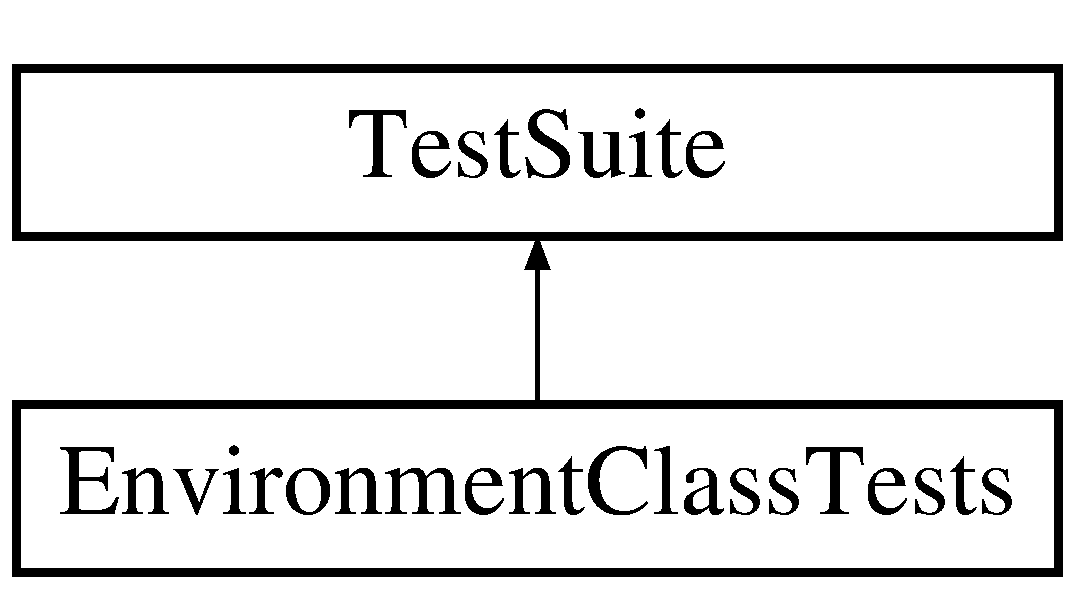
\includegraphics[height=2.000000cm]{classEnvironmentClassTests}
\end{center}
\end{figure}
\subsection*{Public Member Functions}
\begin{DoxyCompactItemize}
\item 
\hypertarget{classEnvironmentClassTests_a62b7cfcf9627301c2b9c54be419f4f42}{void {\bfseries Test\-\_\-\-Sensor} (void)}\label{classEnvironmentClassTests_a62b7cfcf9627301c2b9c54be419f4f42}

\item 
\hypertarget{classEnvironmentClassTests_acc3364a9b7ae1cfc4b02f26aa5595584}{void {\bfseries Test\-\_\-generate\-Rand\-Position} ()}\label{classEnvironmentClassTests_acc3364a9b7ae1cfc4b02f26aa5595584}

\item 
\hypertarget{classEnvironmentClassTests_a9dc861ce2b034e44fe2d3e2d7471fa47}{void {\bfseries Test\-\_\-distance} ()}\label{classEnvironmentClassTests_a9dc861ce2b034e44fe2d3e2d7471fa47}

\end{DoxyCompactItemize}


\subsection{Detailed Description}
environment test for sensor,random position, distance 

The documentation for this class was generated from the following file\-:\begin{DoxyCompactItemize}
\item 
\hyperlink{EnvironmentClassTest_8h}{Environment\-Class\-Test.\-h}\end{DoxyCompactItemize}

\hypertarget{structGLPosition}{\section{G\-L\-Position Struct Reference}
\label{structGLPosition}\index{G\-L\-Position@{G\-L\-Position}}
}


get the G\-Lposition from the struct  




{\ttfamily \#include $<$Common.\-h$>$}

\subsection*{Public Member Functions}
\begin{DoxyCompactItemize}
\item 
\hypertarget{structGLPosition_af1bc843a37986d19db3b497048ca0742}{{\bfseries G\-L\-Position} (G\-Lint x, G\-Lint y, G\-Lint z=0)}\label{structGLPosition_af1bc843a37986d19db3b497048ca0742}

\item 
\hypertarget{structGLPosition_ae678b653b2d3aa648525aab72fec95d6}{\hyperlink{structGLPosition}{G\-L\-Position} \& {\bfseries operator=} (const \hyperlink{structGLPosition}{G\-L\-Position} \&orig)}\label{structGLPosition_ae678b653b2d3aa648525aab72fec95d6}

\item 
\hypertarget{structGLPosition_a96f5cbecf7f65e66a28c36421da65c79}{bool {\bfseries operator!=} (const \hyperlink{structGLPosition}{G\-L\-Position} \&orig)}\label{structGLPosition_a96f5cbecf7f65e66a28c36421da65c79}

\item 
\hypertarget{structGLPosition_a52d0ec6bbc8c0e677d4e16886395025f}{bool {\bfseries operator==} (const \hyperlink{structGLPosition}{G\-L\-Position} \&orig)}\label{structGLPosition_a52d0ec6bbc8c0e677d4e16886395025f}

\end{DoxyCompactItemize}
\subsection*{Public Attributes}
\begin{DoxyCompactItemize}
\item 
\hypertarget{structGLPosition_a282b580759ebed18fc3754d070c12443}{G\-Lint {\bfseries pos\-X}}\label{structGLPosition_a282b580759ebed18fc3754d070c12443}

\item 
\hypertarget{structGLPosition_acea4105d3747c39a6a9feca4c8b1de9b}{G\-Lint {\bfseries pos\-Y}}\label{structGLPosition_acea4105d3747c39a6a9feca4c8b1de9b}

\item 
\hypertarget{structGLPosition_ac54bc083cdad0f7b92337e186c6b6883}{G\-Lint {\bfseries pos\-Z}}\label{structGLPosition_ac54bc083cdad0f7b92337e186c6b6883}

\end{DoxyCompactItemize}


\subsection{Detailed Description}
get the G\-Lposition from the struct 

\begin{DoxyAuthor}{Author}
Jiajun Ni 
\end{DoxyAuthor}


The documentation for this struct was generated from the following file\-:\begin{DoxyCompactItemize}
\item 
\hyperlink{Common_8h}{Common.\-h}\end{DoxyCompactItemize}

\hypertarget{classObject}{\section{Object Class Reference}
\label{classObject}\index{Object@{Object}}
}


base object class obstacle, robot, and any other simulate object.  




{\ttfamily \#include $<$Common.\-h$>$}

Inheritance diagram for Object\-:\begin{figure}[H]
\begin{center}
\leavevmode
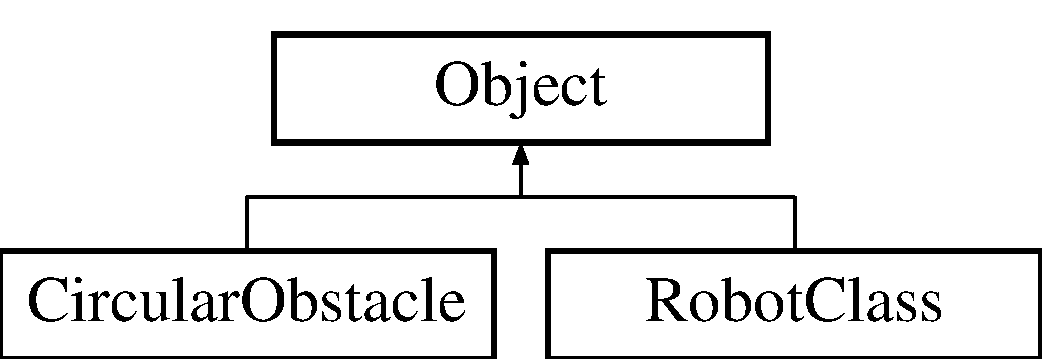
\includegraphics[height=2.000000cm]{classObject}
\end{center}
\end{figure}
\subsection*{Public Types}
\begin{DoxyCompactItemize}
\item 
enum \hyperlink{classObject_ad8dadb365053c182931671a424199e36}{Type} \{ {\bfseries e\-Circular} = 0, 
{\bfseries e\-Plane} = 1, 
{\bfseries e\-Robot} = 2, 
{\bfseries e\-Other}
 \}
\begin{DoxyCompactList}\small\item\em circular obstacle, plane obstacle, robot \end{DoxyCompactList}\end{DoxyCompactItemize}
\subsection*{Public Member Functions}
\begin{DoxyCompactItemize}
\item 
\hypertarget{classObject_a0307ab0a90c744dd7eb65fec04607686}{virtual void \hyperlink{classObject_a0307ab0a90c744dd7eb65fec04607686}{move} (const time\-\_\-t elapsed\-Time)=0}\label{classObject_a0307ab0a90c744dd7eb65fec04607686}

\begin{DoxyCompactList}\small\item\em drive obstacle moving \end{DoxyCompactList}\item 
\hypertarget{classObject_a9f985500da322266d7782ab2cc5e6eaf}{virtual void \hyperlink{classObject_a9f985500da322266d7782ab2cc5e6eaf}{render} (const \hyperlink{Common_8h_a5113b6588451c418d38d8b3681eb6040}{gl\-Color\-Vec} \&c)=0}\label{classObject_a9f985500da322266d7782ab2cc5e6eaf}

\begin{DoxyCompactList}\small\item\em render this object \end{DoxyCompactList}\item 
\hypertarget{classObject_a56f456af2b1ba5a34c27f9b4c5d10dda}{virtual bool \hyperlink{classObject_a56f456af2b1ba5a34c27f9b4c5d10dda}{detect\-Collision} ()=0}\label{classObject_a56f456af2b1ba5a34c27f9b4c5d10dda}

\begin{DoxyCompactList}\small\item\em check if collision with any other object \end{DoxyCompactList}\item 
virtual bool \hyperlink{classObject_abba9760277a437884404992f926d2e4d}{detect\-Overlapping} (\hyperlink{structGLPosition}{G\-L\-Position} \&pos\-Left\-Top, \hyperlink{structGLPosition}{G\-L\-Position} \&pos\-Right\-Bottom, const G\-Lint \&radius)
\begin{DoxyCompactList}\small\item\em check if over lapped with any other object? \end{DoxyCompactList}\item 
virtual bool \hyperlink{classObject_ad9adac7de77247bd045a43c317794899}{detect\-Wall} (const G\-Lint \&width, const G\-Lint \&height, const G\-Lint \&radius) const 
\begin{DoxyCompactList}\small\item\em check if collided with wall? \end{DoxyCompactList}\end{DoxyCompactItemize}
\subsection*{Protected Member Functions}
\begin{DoxyCompactItemize}
\item 
\hypertarget{classObject_a59f4160d4d035e85ebdd706acdcd60f9}{virtual void \hyperlink{classObject_a59f4160d4d035e85ebdd706acdcd60f9}{draw} ()=0}\label{classObject_a59f4160d4d035e85ebdd706acdcd60f9}

\begin{DoxyCompactList}\small\item\em draw this object \end{DoxyCompactList}\end{DoxyCompactItemize}


\subsection{Detailed Description}
base object class obstacle, robot, and any other simulate object. 

\begin{DoxyAuthor}{Author}
Jiajun Ni 
\end{DoxyAuthor}


\subsection{Member Function Documentation}
\hypertarget{classObject_abba9760277a437884404992f926d2e4d}{\index{Object@{Object}!detect\-Overlapping@{detect\-Overlapping}}
\index{detect\-Overlapping@{detect\-Overlapping}!Object@{Object}}
\subsubsection[{detect\-Overlapping}]{\setlength{\rightskip}{0pt plus 5cm}bool Object\-::detect\-Overlapping (
\begin{DoxyParamCaption}
\item[{{\bf G\-L\-Position} \&}]{pos\-Left\-Top, }
\item[{{\bf G\-L\-Position} \&}]{pos\-Right\-Bottom, }
\item[{const G\-Lint \&}]{radius}
\end{DoxyParamCaption}
)\hspace{0.3cm}{\ttfamily [virtual]}}}\label{classObject_abba9760277a437884404992f926d2e4d}


check if over lapped with any other object? 

avoid overlapping

\begin{DoxyAuthor}{Author}
Jiajun Ni 
\end{DoxyAuthor}

\begin{DoxyParams}{Parameters}
{\em pos\-Left\-Top} & \\
\hline
{\em pos\-Right\-Bottom} & \\
\hline
\end{DoxyParams}

\begin{DoxyCode}
 arrange data of the rectangle
 /
\textcolor{keywordtype}{float} dist;
\textcolor{keywordflow}{if} (posLeftTop.posX > posRightBottom.posX)
\{
    dist = posRightBottom.posX;
    posRightBottom.posX = posLeftTop.posX;
    posLeftTop.posX = dist;
\}
\textcolor{keywordflow}{if} (posLeftTop.posY > posRightBottom.posY)
\{
    dist = posRightBottom.posY;
    posRightBottom.posY = posLeftTop.posY;
    posLeftTop.posY = dist;
\}
\end{DoxyCode}



\begin{DoxyCode}
  check whether inscribed square of the cirle and the rectangle cross,
  express the inscribed square with four line which can be expressed by a number
 /
dist = radius / (float)1.4142136;

\textcolor{keywordtype}{float} xSquare1 = position.posX - dist;
\textcolor{keywordtype}{float} xSquare2 = position.posX + dist;
\textcolor{keywordtype}{float} ySquare1 = position.posY - dist;
\textcolor{keywordtype}{float} ySquare2 = position.posY + dist;

\textcolor{keywordflow}{if} (xSquare1 <= posRightBottom.posX && xSquare2 >= posLeftTop.posX && ySquare1 <= posLeftTop.posY
    && ySquare2 >= posRightBottom.posY)
\{
    \textcolor{keywordflow}{return} \textcolor{keyword}{true};
\}
\end{DoxyCode}



\begin{DoxyCode}
 check whether there is a vertex of the rectangle in the circle position of rectangle
 /
\textcolor{keywordtype}{float} xrectangle = (posLeftTop.posX + posRightBottom.posX) / 2;
\textcolor{keywordtype}{float} yrectangle = (posLeftTop.posY + posRightBottom.posY) / 2;
\textcolor{comment}{/**}
\end{DoxyCode}



\begin{DoxyCode}
 rectangle is on the top left side of circle*/
\textcolor{keywordflow}{if} (xrectangle <= position.posX && yrectangle <= position.posY
    && sqrt((posRightBottom.posX - position.posX) * (posRightBottom.posX - position.posX) + (posRightBottom
      .posY - position.posY) *
    (posRightBottom.posY - position.posY)) <= radius)
    \textcolor{keywordflow}{return} \textcolor{keyword}{true};
\textcolor{keywordflow}{else} \textcolor{keywordflow}{if} (xrectangle > position.posX && yrectangle <= position.posY
    && sqrt((posLeftTop.posX - position.posX) * (posLeftTop.posX - position.posX) + (posRightBottom.posY - 
      position.posY) *
    (posRightBottom.posY - position.posY)) <= radius)
    \textcolor{keywordflow}{return} \textcolor{keyword}{true};
\textcolor{keywordflow}{else} \textcolor{keywordflow}{if} (xrectangle <= position.posX && yrectangle > position.posY
    && sqrt((posRightBottom.posX - position.posX) * (posRightBottom.posX - position.posX) + (posLeftTop.
      posY - position.posY) *
    (posLeftTop.posY - position.posY)) <= radius)
    \textcolor{keywordflow}{return} \textcolor{keyword}{true};
\textcolor{keywordflow}{else} \textcolor{keywordflow}{if} (sqrt((posLeftTop.posX - position.posX) * (posLeftTop.posX - position.posX) + (posLeftTop.posY - 
      position.posY) *
    (posLeftTop.posY - position.posY)) <= radius)
    \textcolor{keywordflow}{return} \textcolor{keyword}{true};
\end{DoxyCode}



\begin{DoxyCode}
 check whether there is one of the four points of the circle is in the rectangle*/
\textcolor{keywordflow}{if} (((position.posX - radius >= posLeftTop.posX && position.posX - radius <= posRightBottom.posX) ||
    (position.posX + radius >= posLeftTop.posX && position.posX + radius <= posRightBottom.posX))
    && position.posY >= posLeftTop.posY && position.posY <= posRightBottom.posY ||
    ((position.posY - radius >= posLeftTop.posY && position.posY - radius >= posRightBottom.posY) ||
    (position.posY + radius >= posLeftTop.posY && position.posY + radius <= posRightBottom.posY)) &&
    position.posX >= posLeftTop.posX && position.posX <= posRightBottom.posX)
\{
    \textcolor{keywordflow}{return} \textcolor{keyword}{true};
\}
\end{DoxyCode}


no case match \hypertarget{classObject_ad9adac7de77247bd045a43c317794899}{\index{Object@{Object}!detect\-Wall@{detect\-Wall}}
\index{detect\-Wall@{detect\-Wall}!Object@{Object}}
\subsubsection[{detect\-Wall}]{\setlength{\rightskip}{0pt plus 5cm}bool Object\-::detect\-Wall (
\begin{DoxyParamCaption}
\item[{const G\-Lint \&}]{width, }
\item[{const G\-Lint \&}]{height, }
\item[{const G\-Lint \&}]{radius}
\end{DoxyParamCaption}
) const\hspace{0.3cm}{\ttfamily [virtual]}}}\label{classObject_ad9adac7de77247bd045a43c317794899}


check if collided with wall? 

detect\-Wall.

\begin{DoxyAuthor}{Author}
Jiajun Ni 
\end{DoxyAuthor}

\begin{DoxyParams}{Parameters}
{\em width} & the width of the window \\
\hline
{\em height} & the height of the window \\
\hline
\end{DoxyParams}


The documentation for this class was generated from the following files\-:\begin{DoxyCompactItemize}
\item 
\hyperlink{Common_8h}{Common.\-h}\item 
Common.\-cpp\end{DoxyCompactItemize}

\hypertarget{classObstacleTests}{\section{Obstacle\-Tests Class Reference}
\label{classObstacleTests}\index{Obstacle\-Tests@{Obstacle\-Tests}}
}


test for the obstacle's basic attributes  




{\ttfamily \#include $<$Obstacle\-Test.\-h$>$}

Inheritance diagram for Obstacle\-Tests\-:\begin{figure}[H]
\begin{center}
\leavevmode
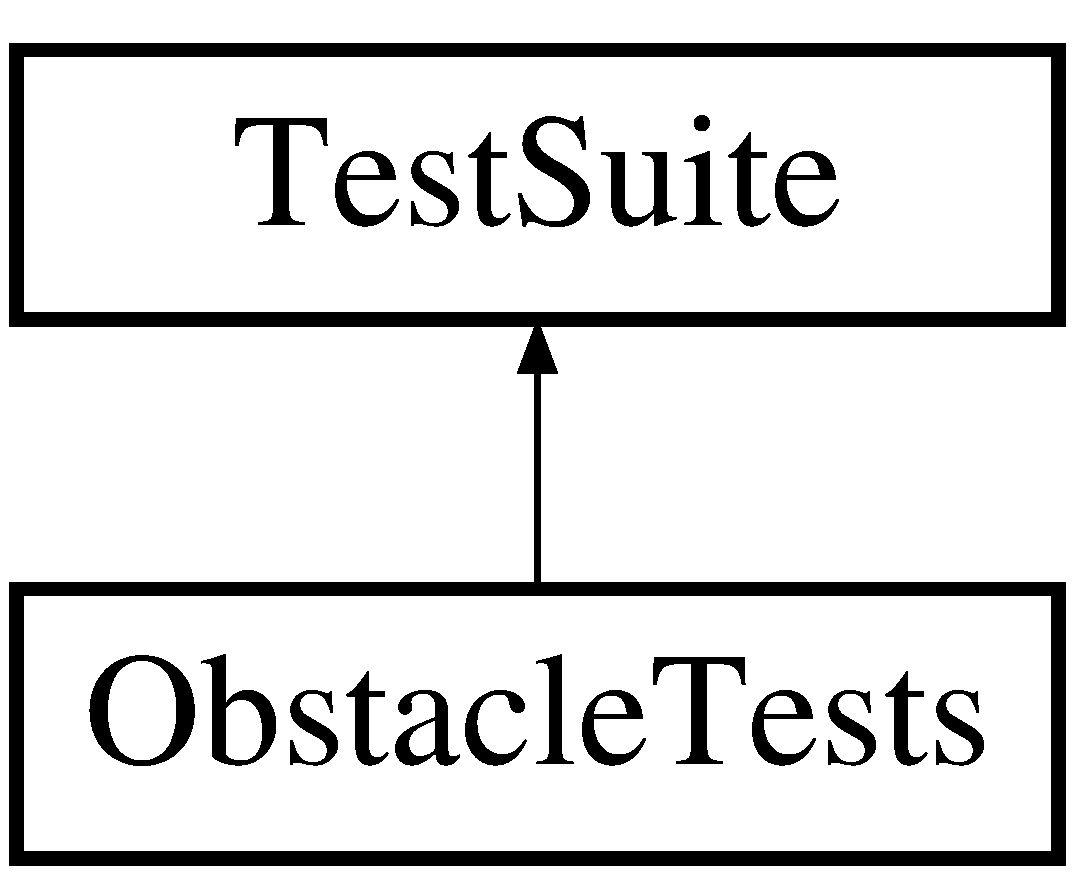
\includegraphics[height=2.000000cm]{classObstacleTests}
\end{center}
\end{figure}
\subsection*{Public Member Functions}
\begin{DoxyCompactItemize}
\item 
\hypertarget{classObstacleTests_ae8fd342ec510c6a32d8bd9464e34c11b}{void {\bfseries Test\-\_\-move} ()}\label{classObstacleTests_ae8fd342ec510c6a32d8bd9464e34c11b}

\item 
\hypertarget{classObstacleTests_a13d6e2e50cb059f41434e01e02e883e0}{void {\bfseries Test\-\_\-render} ()}\label{classObstacleTests_a13d6e2e50cb059f41434e01e02e883e0}

\item 
\hypertarget{classObstacleTests_a282fe4485426b3f277d5cb6cf32405ba}{void {\bfseries Test\-\_\-rotate} ()}\label{classObstacleTests_a282fe4485426b3f277d5cb6cf32405ba}

\item 
\hypertarget{classObstacleTests_a314341e9bdcdcd2fa2e73b51fdfcd07d}{void {\bfseries Test\-\_\-radious} ()}\label{classObstacleTests_a314341e9bdcdcd2fa2e73b51fdfcd07d}

\item 
\hypertarget{classObstacleTests_a11369ab95a22d9ae1a80097aff6023a1}{void {\bfseries Test\-\_\-color} ()}\label{classObstacleTests_a11369ab95a22d9ae1a80097aff6023a1}

\end{DoxyCompactItemize}


\subsection{Detailed Description}
test for the obstacle's basic attributes 

The documentation for this class was generated from the following file\-:\begin{DoxyCompactItemize}
\item 
\hyperlink{ObstacleTest_8h}{Obstacle\-Test.\-h}\end{DoxyCompactItemize}

\hypertarget{classRobotClass}{\section{Robot\-Class Class Reference}
\label{classRobotClass}\index{Robot\-Class@{Robot\-Class}}
}


\hyperlink{classRobotClass}{Robot\-Class}. This provides means to store and alter robot state.  




{\ttfamily \#include $<$Robot\-Class.\-h$>$}

Inheritance diagram for Robot\-Class\-:\begin{figure}[H]
\begin{center}
\leavevmode
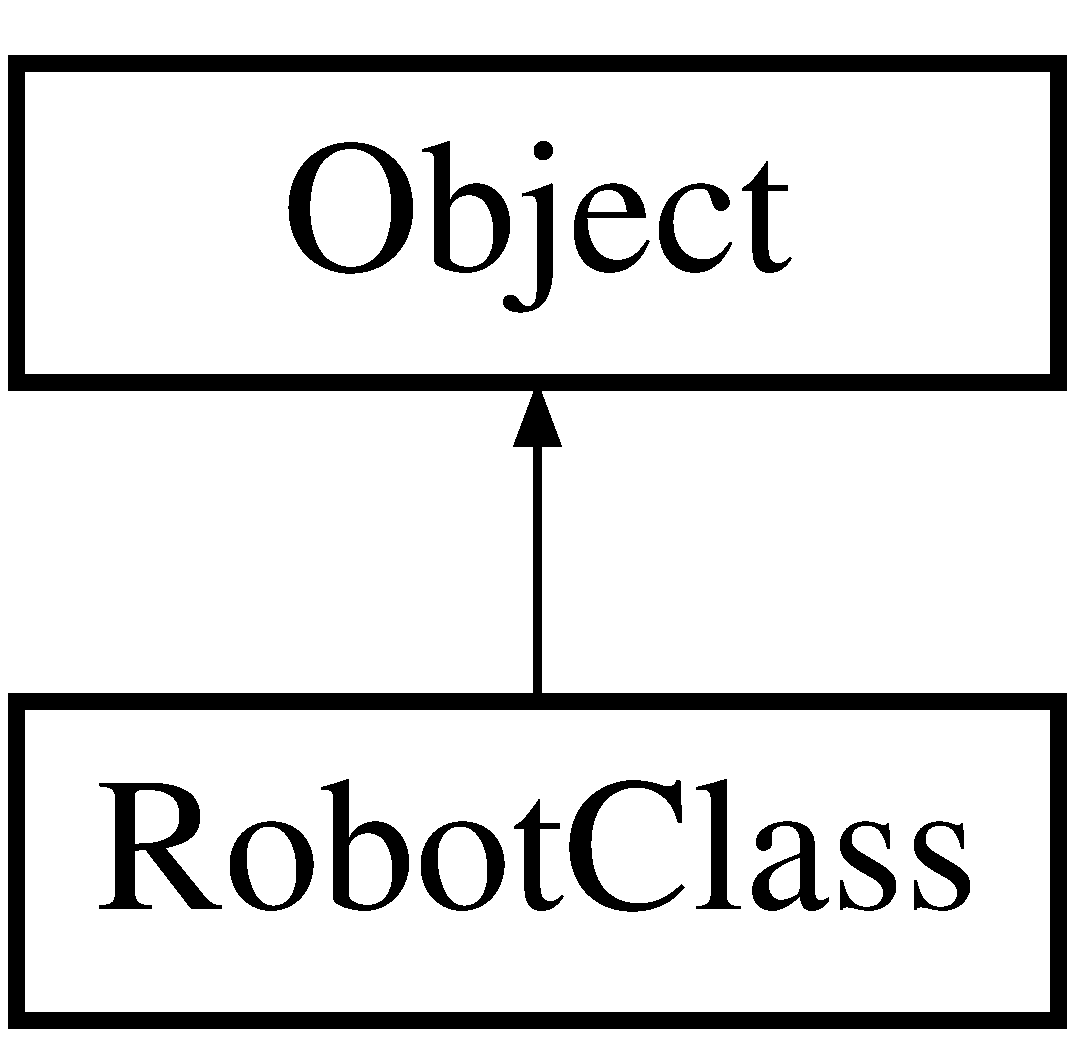
\includegraphics[height=2.000000cm]{classRobotClass}
\end{center}
\end{figure}
\subsection*{Public Member Functions}
\begin{DoxyCompactItemize}
\item 
\hyperlink{classRobotClass_a7125604039c2a4b39e34e4354bd4ce19}{Robot\-Class} ()
\begin{DoxyCompactList}\small\item\em initialize the position, radius, direction. \end{DoxyCompactList}\item 
\hyperlink{classRobotClass_ae38ea864dfa0cc63e64a33f33334d804}{Robot\-Class} (\hyperlink{structGLPosition}{G\-L\-Position} \&pos, G\-Lint r, G\-Lint d)
\begin{DoxyCompactList}\small\item\em current position, radius, direction. \end{DoxyCompactList}\item 
void \hyperlink{classRobotClass_a83fc8dd757868ab599208245e3aa04cb}{set\-Orientation} (const G\-Lint \&degrees)
\begin{DoxyCompactList}\small\item\em orientation in degrees G\-Lint \hyperlink{classRobotClass_a808e1643328178e9b0742bab2480d2d4}{get\-Orientation()},speed in pixels per second \end{DoxyCompactList}\item 
G\-Lint \hyperlink{classRobotClass_a808e1643328178e9b0742bab2480d2d4}{get\-Orientation} ()
\begin{DoxyCompactList}\small\item\em get orientation of robot \end{DoxyCompactList}\item 
void \hyperlink{classRobotClass_ada07c364411e6d4c3efd6c5f5e4e6275}{set\-Speed} (const G\-Lint \&pps)
\begin{DoxyCompactList}\small\item\em set the speed of robot. The speed cannot be less than 0. Set the speed to null when input less that 0. \end{DoxyCompactList}\item 
G\-Lint \hyperlink{classRobotClass_ac39e7492ee082cb36818f93845c75983}{get\-Speed} ()
\begin{DoxyCompactList}\small\item\em get speed of robot \end{DoxyCompactList}\item 
\hypertarget{classRobotClass_a1fbee3e9632e92bb6cde8ef3db4ce9eb}{void {\bfseries set\-Direction\-Color} (const \hyperlink{Common_8h_a5113b6588451c418d38d8b3681eb6040}{gl\-Color\-Vec} \&color)}\label{classRobotClass_a1fbee3e9632e92bb6cde8ef3db4ce9eb}

\item 
\hypertarget{classRobotClass_adcdf87caada18aeca7ee43b73a1f3010}{\hyperlink{Common_8h_a5113b6588451c418d38d8b3681eb6040}{gl\-Color\-Vec} {\bfseries direction\-Color} ()}\label{classRobotClass_adcdf87caada18aeca7ee43b73a1f3010}

\item 
\hypertarget{classRobotClass_a364ac0f9c65a4c2ee4d5b73a09f3ab34}{virtual void \hyperlink{classRobotClass_a364ac0f9c65a4c2ee4d5b73a09f3ab34}{move} (const time\-\_\-t elapsed\-Time)}\label{classRobotClass_a364ac0f9c65a4c2ee4d5b73a09f3ab34}

\begin{DoxyCompactList}\small\item\em drive obstacle moving \end{DoxyCompactList}\item 
\hypertarget{classRobotClass_af2069bec3bb391b05676e154527674fa}{virtual void \hyperlink{classRobotClass_af2069bec3bb391b05676e154527674fa}{render} (const \hyperlink{Common_8h_a5113b6588451c418d38d8b3681eb6040}{gl\-Color\-Vec} \&c)}\label{classRobotClass_af2069bec3bb391b05676e154527674fa}

\begin{DoxyCompactList}\small\item\em render this object \end{DoxyCompactList}\item 
\hypertarget{classRobotClass_a723bf7484fefcc8860e606d9041f9c76}{void {\bfseries set\-Target} (const int \&id)}\label{classRobotClass_a723bf7484fefcc8860e606d9041f9c76}

\item 
\hypertarget{classRobotClass_ab8e01362440cf6a0b5eaa6deaceb1c5e}{int {\bfseries target} () const }\label{classRobotClass_ab8e01362440cf6a0b5eaa6deaceb1c5e}

\item 
\hypertarget{classRobotClass_a805c3afc1be17e30b228d33df3e194e8}{void {\bfseries rotate} (const G\-Lint \&deg)}\label{classRobotClass_a805c3afc1be17e30b228d33df3e194e8}

\item 
\hypertarget{classRobotClass_affdee45ae76e3408db1c1615439b5b02}{void {\bfseries update\-Position} (const \hyperlink{structGLPosition}{G\-L\-Position} \&new\-Pos)}\label{classRobotClass_affdee45ae76e3408db1c1615439b5b02}

\item 
\hypertarget{classRobotClass_a1df74eb30a5bda3025eecd188ad42c54}{bool \hyperlink{classRobotClass_a1df74eb30a5bda3025eecd188ad42c54}{detect\-Collision} ()}\label{classRobotClass_a1df74eb30a5bda3025eecd188ad42c54}

\begin{DoxyCompactList}\small\item\em check if collision with any other object \end{DoxyCompactList}\item 
G\-Lint \hyperlink{classRobotClass_a61a9c5217fb1092668c55864b7e4bad0}{get\-Radius} () const 
\end{DoxyCompactItemize}
\subsection*{Public Attributes}
\begin{DoxyCompactItemize}
\item 
\hypertarget{classRobotClass_ad1c37dd20e2049c9f083d44ab05f34e2}{\hyperlink{Common_8h_a5113b6588451c418d38d8b3681eb6040}{gl\-Color\-Vec} {\bfseries color}}\label{classRobotClass_ad1c37dd20e2049c9f083d44ab05f34e2}

\item 
\hypertarget{classRobotClass_a34bfb4f398462a875ec7f1f213beb6f1}{int {\bfseries collided}}\label{classRobotClass_a34bfb4f398462a875ec7f1f213beb6f1}

\end{DoxyCompactItemize}
\subsection*{Protected Member Functions}
\begin{DoxyCompactItemize}
\item 
virtual void \hyperlink{classRobotClass_af49350c7e914e11df672cc9de68c9ff1}{draw} ()
\begin{DoxyCompactList}\small\item\em draw a circle represent the robot and a line represent the direction. \end{DoxyCompactList}\item 
bool \hyperlink{classRobotClass_a480964a3187868d543c0c1f1cf998162}{detect\-Obstacle} (const \hyperlink{classObject}{Object} $\ast$p\-Obj)
\begin{DoxyCompactList}\small\item\em detect\-Obstacle \end{DoxyCompactList}\end{DoxyCompactItemize}
\subsection*{Friends}
\begin{DoxyCompactItemize}
\item 
\hypertarget{classRobotClass_a02448c8c195e97f3229c6803f47bf8d7}{class {\bfseries Robot\-Tests}}\label{classRobotClass_a02448c8c195e97f3229c6803f47bf8d7}

\end{DoxyCompactItemize}
\subsection*{Additional Inherited Members}


\subsection{Detailed Description}
\hyperlink{classRobotClass}{Robot\-Class}. This provides means to store and alter robot state. 

\subsection{Constructor \& Destructor Documentation}
\hypertarget{classRobotClass_a7125604039c2a4b39e34e4354bd4ce19}{\index{Robot\-Class@{Robot\-Class}!Robot\-Class@{Robot\-Class}}
\index{Robot\-Class@{Robot\-Class}!RobotClass@{Robot\-Class}}
\subsubsection[{Robot\-Class}]{\setlength{\rightskip}{0pt plus 5cm}Robot\-Class\-::\-Robot\-Class (
\begin{DoxyParamCaption}
{}
\end{DoxyParamCaption}
)}}\label{classRobotClass_a7125604039c2a4b39e34e4354bd4ce19}


initialize the position, radius, direction. 

\begin{DoxyAuthor}{Author}
Jiajun Ni 
\end{DoxyAuthor}
\hypertarget{classRobotClass_ae38ea864dfa0cc63e64a33f33334d804}{\index{Robot\-Class@{Robot\-Class}!Robot\-Class@{Robot\-Class}}
\index{Robot\-Class@{Robot\-Class}!RobotClass@{Robot\-Class}}
\subsubsection[{Robot\-Class}]{\setlength{\rightskip}{0pt plus 5cm}Robot\-Class\-::\-Robot\-Class (
\begin{DoxyParamCaption}
\item[{{\bf G\-L\-Position} \&}]{pos, }
\item[{G\-Lint}]{r, }
\item[{G\-Lint}]{d}
\end{DoxyParamCaption}
)}}\label{classRobotClass_ae38ea864dfa0cc63e64a33f33334d804}


current position, radius, direction. 

\begin{DoxyAuthor}{Author}
Jiajun Ni 
\end{DoxyAuthor}

\begin{DoxyParams}{Parameters}
{\em pos} & the position \\
\hline
{\em r} & the radius \\
\hline
{\em d} & the direction \\
\hline
\end{DoxyParams}


\subsection{Member Function Documentation}
\hypertarget{classRobotClass_a480964a3187868d543c0c1f1cf998162}{\index{Robot\-Class@{Robot\-Class}!detect\-Obstacle@{detect\-Obstacle}}
\index{detect\-Obstacle@{detect\-Obstacle}!RobotClass@{Robot\-Class}}
\subsubsection[{detect\-Obstacle}]{\setlength{\rightskip}{0pt plus 5cm}bool Robot\-Class\-::detect\-Obstacle (
\begin{DoxyParamCaption}
\item[{const {\bf Object} $\ast$}]{p\-Obj}
\end{DoxyParamCaption}
)\hspace{0.3cm}{\ttfamily [protected]}}}\label{classRobotClass_a480964a3187868d543c0c1f1cf998162}


detect\-Obstacle 

\begin{DoxyAuthor}{Author}
Jiajun Ni 
\end{DoxyAuthor}

\begin{DoxyParams}{Parameters}
{\em p\-Obs} & position of the Obstacles \\
\hline
\end{DoxyParams}
\hypertarget{classRobotClass_af49350c7e914e11df672cc9de68c9ff1}{\index{Robot\-Class@{Robot\-Class}!draw@{draw}}
\index{draw@{draw}!RobotClass@{Robot\-Class}}
\subsubsection[{draw}]{\setlength{\rightskip}{0pt plus 5cm}void Robot\-Class\-::draw (
\begin{DoxyParamCaption}
{}
\end{DoxyParamCaption}
)\hspace{0.3cm}{\ttfamily [protected]}, {\ttfamily [virtual]}}}\label{classRobotClass_af49350c7e914e11df672cc9de68c9ff1}


draw a circle represent the robot and a line represent the direction. 

\begin{DoxyAuthor}{Author}
Jiajun Ni 
\end{DoxyAuthor}

\begin{DoxyCode}
  \hyperlink{classRobotClass_af49350c7e914e11df672cc9de68c9ff1}{draw} a circle(robot)
  and a line for direction
  /
for (\textcolor{keywordtype}{int} i = 0; i <= sections; i++)
\{
    glVertex2f(position.posX + radius * cos(i * TWOPI / sections), position.posY + radius * sin(i * TWOPI /
       sections));
\}

glEnd();

GLint length = radius + 5;

glColor3f(direColor.posX, direColor.posY, direColor.posZ);
glBegin(GL\_LINE\_STRIP);

glVertex2d(position.posX, position.posY);
glVertex2d(position.posX + length * cos(direction * PI / 180), position.posY + length * sin(direction * PI 
      / 180));

glEnd();
\end{DoxyCode}
 

Implements \hyperlink{classObject_a59f4160d4d035e85ebdd706acdcd60f9}{Object}.

\hypertarget{classRobotClass_a808e1643328178e9b0742bab2480d2d4}{\index{Robot\-Class@{Robot\-Class}!get\-Orientation@{get\-Orientation}}
\index{get\-Orientation@{get\-Orientation}!RobotClass@{Robot\-Class}}
\subsubsection[{get\-Orientation}]{\setlength{\rightskip}{0pt plus 5cm}G\-Lint Robot\-Class\-::get\-Orientation (
\begin{DoxyParamCaption}
{}
\end{DoxyParamCaption}
)}}\label{classRobotClass_a808e1643328178e9b0742bab2480d2d4}


get orientation of robot 

\begin{DoxyAuthor}{Author}
Jiajun Ni 
\end{DoxyAuthor}
\hypertarget{classRobotClass_a61a9c5217fb1092668c55864b7e4bad0}{\index{Robot\-Class@{Robot\-Class}!get\-Radius@{get\-Radius}}
\index{get\-Radius@{get\-Radius}!RobotClass@{Robot\-Class}}
\subsubsection[{get\-Radius}]{\setlength{\rightskip}{0pt plus 5cm}G\-Lint Robot\-Class\-::get\-Radius (
\begin{DoxyParamCaption}
{}
\end{DoxyParamCaption}
) const}}\label{classRobotClass_a61a9c5217fb1092668c55864b7e4bad0}

\begin{DoxyCode}
   setup the movement \textcolor{keywordflow}{for} robot
  /
\textcolor{keywordtype}{void} \hyperlink{classRobotClass_a364ac0f9c65a4c2ee4d5b73a09f3ab34}{RobotClass::move}(\textcolor{keyword}{const} time\_t elapsedTime)
\{
    GLint distance = elapsedTime * speed;
    \hyperlink{structGLPosition}{GLPosition} nextPos =
        \hyperlink{structGLPosition}{GLPosition}(position.posX + distance * cos(direction * PI / 180), position.posY + distance
       * sin(direction * PI / 180), 0);
        
    \hyperlink{classRobotClass_af49350c7e914e11df672cc9de68c9ff1}{draw}();
    updatePosition(nextPos);
\}
\end{DoxyCode}
 \hypertarget{classRobotClass_ac39e7492ee082cb36818f93845c75983}{\index{Robot\-Class@{Robot\-Class}!get\-Speed@{get\-Speed}}
\index{get\-Speed@{get\-Speed}!RobotClass@{Robot\-Class}}
\subsubsection[{get\-Speed}]{\setlength{\rightskip}{0pt plus 5cm}G\-Lint Robot\-Class\-::get\-Speed (
\begin{DoxyParamCaption}
{}
\end{DoxyParamCaption}
)}}\label{classRobotClass_ac39e7492ee082cb36818f93845c75983}


get speed of robot 

\begin{DoxyAuthor}{Author}
Jiajun Ni 
\end{DoxyAuthor}
\hypertarget{classRobotClass_a83fc8dd757868ab599208245e3aa04cb}{\index{Robot\-Class@{Robot\-Class}!set\-Orientation@{set\-Orientation}}
\index{set\-Orientation@{set\-Orientation}!RobotClass@{Robot\-Class}}
\subsubsection[{set\-Orientation}]{\setlength{\rightskip}{0pt plus 5cm}void Robot\-Class\-::set\-Orientation (
\begin{DoxyParamCaption}
\item[{const G\-Lint \&}]{degrees}
\end{DoxyParamCaption}
)}}\label{classRobotClass_a83fc8dd757868ab599208245e3aa04cb}


orientation in degrees G\-Lint \hyperlink{classRobotClass_a808e1643328178e9b0742bab2480d2d4}{get\-Orientation()},speed in pixels per second 

set the orientation of robot.

\begin{DoxyAuthor}{Author}
Jiajun Ni 
\end{DoxyAuthor}

\begin{DoxyParams}{Parameters}
{\em degree} & the direction \\
\hline
\end{DoxyParams}
\hypertarget{classRobotClass_ada07c364411e6d4c3efd6c5f5e4e6275}{\index{Robot\-Class@{Robot\-Class}!set\-Speed@{set\-Speed}}
\index{set\-Speed@{set\-Speed}!RobotClass@{Robot\-Class}}
\subsubsection[{set\-Speed}]{\setlength{\rightskip}{0pt plus 5cm}void Robot\-Class\-::set\-Speed (
\begin{DoxyParamCaption}
\item[{const G\-Lint \&}]{pps}
\end{DoxyParamCaption}
)}}\label{classRobotClass_ada07c364411e6d4c3efd6c5f5e4e6275}


set the speed of robot. The speed cannot be less than 0. Set the speed to null when input less that 0. 

\begin{DoxyAuthor}{Author}
Jiajun Ni, Jiajun Ni 
\end{DoxyAuthor}

\begin{DoxyParams}{Parameters}
{\em pps} & speed \\
\hline
\end{DoxyParams}


The documentation for this class was generated from the following files\-:\begin{DoxyCompactItemize}
\item 
\hyperlink{RobotClass_8h}{Robot\-Class.\-h}\item 
\hyperlink{RobotClass_8cpp}{Robot\-Class.\-cpp}\end{DoxyCompactItemize}

\hypertarget{classRobotTests}{\section{Robot\-Tests Class Reference}
\label{classRobotTests}\index{Robot\-Tests@{Robot\-Tests}}
}


Test robot's position,orientation, speed, movement and the detection of obstacle.  




{\ttfamily \#include $<$Robot\-Tests.\-h$>$}

Inheritance diagram for Robot\-Tests\-:\begin{figure}[H]
\begin{center}
\leavevmode
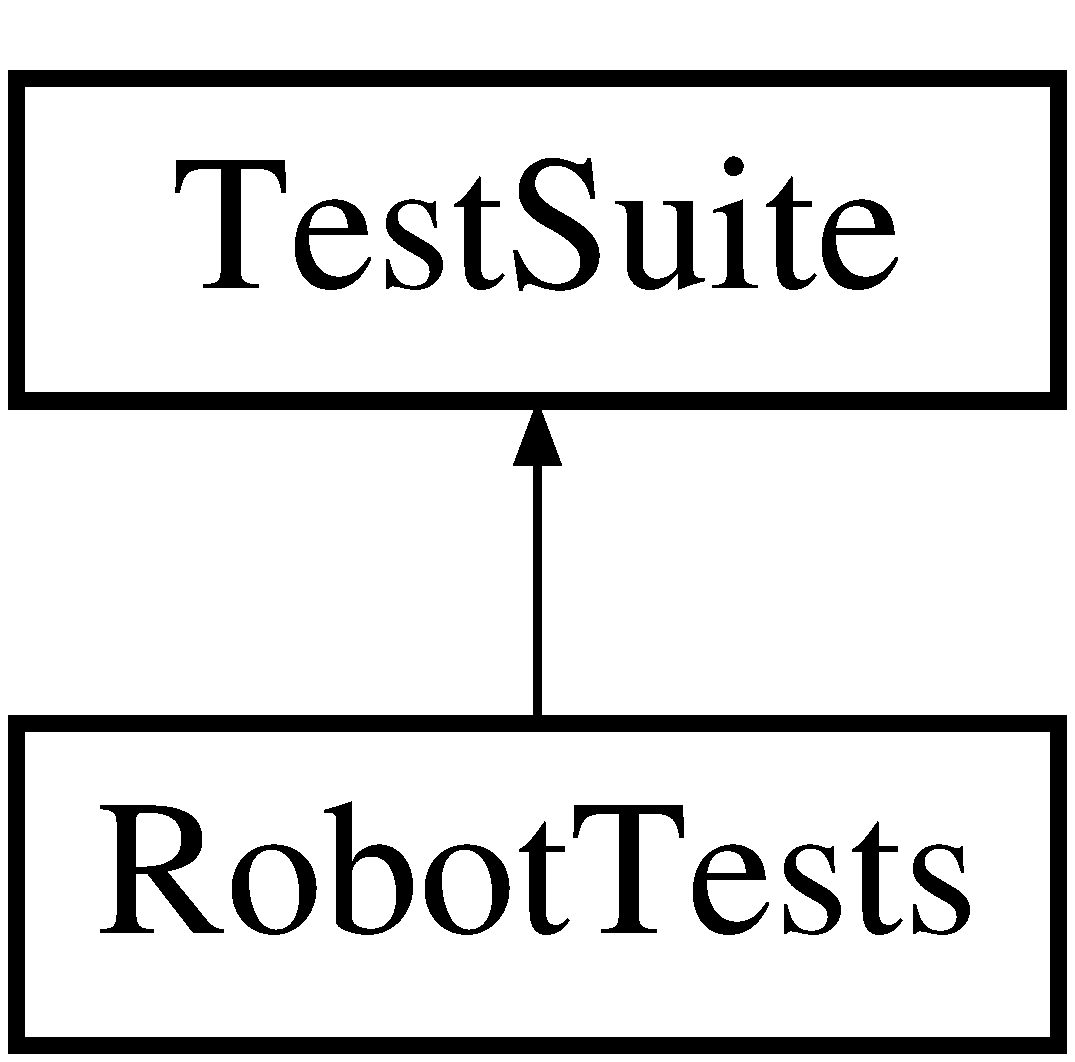
\includegraphics[height=2.000000cm]{classRobotTests}
\end{center}
\end{figure}
\subsection*{Public Member Functions}
\begin{DoxyCompactItemize}
\item 
void \hyperlink{classRobotTests_ac6a7dfed3f30380ec2e85759d8d4808c}{Test\-\_\-\-Position} (void)
\item 
void \hyperlink{classRobotTests_aca7125d3b2733b1b30bed1857c5a97f6}{Test\-\_\-\-Orientation} (void)
\item 
void \hyperlink{classRobotTests_a6d724a2821a085331c532fe1b189d0fc}{test\-\_\-\-Speed} (void)
\item 
\hypertarget{classRobotTests_a5dfdc3ca971f35cf23ddb1a8e364f90a}{void {\bfseries Test\-\_\-move} ()}\label{classRobotTests_a5dfdc3ca971f35cf23ddb1a8e364f90a}

\item 
void \hyperlink{classRobotTests_ae5de21633b1944c8c54b047b6a4982eb}{test\-\_\-detect\-Obstacle} (void)
\item 
\hypertarget{classRobotTests_a9f7fb0d82ad18249333f9b9ab37e6528}{void {\bfseries test\-\_\-display} (void)}\label{classRobotTests_a9f7fb0d82ad18249333f9b9ab37e6528}

\item 
\hypertarget{classRobotTests_a74b1812b3a6a464e070ef6203cb44118}{void {\bfseries test\-\_\-left\-Mouse\-Down} (void)}\label{classRobotTests_a74b1812b3a6a464e070ef6203cb44118}

\item 
\hypertarget{classRobotTests_a96009755981485df4f2df50ef2bd4243}{void {\bfseries test\-\_\-left\-Mouse\-Up} (void)}\label{classRobotTests_a96009755981485df4f2df50ef2bd4243}

\end{DoxyCompactItemize}


\subsection{Detailed Description}
Test robot's position,orientation, speed, movement and the detection of obstacle. 

\subsection{Member Function Documentation}
\hypertarget{classRobotTests_ae5de21633b1944c8c54b047b6a4982eb}{\index{Robot\-Tests@{Robot\-Tests}!test\-\_\-detect\-Obstacle@{test\-\_\-detect\-Obstacle}}
\index{test\-\_\-detect\-Obstacle@{test\-\_\-detect\-Obstacle}!RobotTests@{Robot\-Tests}}
\subsubsection[{test\-\_\-detect\-Obstacle}]{\setlength{\rightskip}{0pt plus 5cm}void Robot\-Tests\-::test\-\_\-detect\-Obstacle (
\begin{DoxyParamCaption}
\item[{void}]{}
\end{DoxyParamCaption}
)\hspace{0.3cm}{\ttfamily [inline]}}}\label{classRobotTests_ae5de21633b1944c8c54b047b6a4982eb}
\begin{DoxyAuthor}{Author}
Robin Holtman 
\end{DoxyAuthor}
Robot inside obstacle \hypertarget{classRobotTests_aca7125d3b2733b1b30bed1857c5a97f6}{\index{Robot\-Tests@{Robot\-Tests}!Test\-\_\-\-Orientation@{Test\-\_\-\-Orientation}}
\index{Test\-\_\-\-Orientation@{Test\-\_\-\-Orientation}!RobotTests@{Robot\-Tests}}
\subsubsection[{Test\-\_\-\-Orientation}]{\setlength{\rightskip}{0pt plus 5cm}void Robot\-Tests\-::\-Test\-\_\-\-Orientation (
\begin{DoxyParamCaption}
\item[{void}]{}
\end{DoxyParamCaption}
)\hspace{0.3cm}{\ttfamily [inline]}}}\label{classRobotTests_aca7125d3b2733b1b30bed1857c5a97f6}
\begin{DoxyAuthor}{Author}
Jiajun Ni 
\end{DoxyAuthor}
\hypertarget{classRobotTests_ac6a7dfed3f30380ec2e85759d8d4808c}{\index{Robot\-Tests@{Robot\-Tests}!Test\-\_\-\-Position@{Test\-\_\-\-Position}}
\index{Test\-\_\-\-Position@{Test\-\_\-\-Position}!RobotTests@{Robot\-Tests}}
\subsubsection[{Test\-\_\-\-Position}]{\setlength{\rightskip}{0pt plus 5cm}void Robot\-Tests\-::\-Test\-\_\-\-Position (
\begin{DoxyParamCaption}
\item[{void}]{}
\end{DoxyParamCaption}
)\hspace{0.3cm}{\ttfamily [inline]}}}\label{classRobotTests_ac6a7dfed3f30380ec2e85759d8d4808c}
\begin{DoxyAuthor}{Author}
Jiajun Ni 
\end{DoxyAuthor}
\hypertarget{classRobotTests_a6d724a2821a085331c532fe1b189d0fc}{\index{Robot\-Tests@{Robot\-Tests}!test\-\_\-\-Speed@{test\-\_\-\-Speed}}
\index{test\-\_\-\-Speed@{test\-\_\-\-Speed}!RobotTests@{Robot\-Tests}}
\subsubsection[{test\-\_\-\-Speed}]{\setlength{\rightskip}{0pt plus 5cm}void Robot\-Tests\-::test\-\_\-\-Speed (
\begin{DoxyParamCaption}
\item[{void}]{}
\end{DoxyParamCaption}
)\hspace{0.3cm}{\ttfamily [inline]}}}\label{classRobotTests_a6d724a2821a085331c532fe1b189d0fc}
\begin{DoxyAuthor}{Author}
Jiajun Ni, Xinyue Zhang 
\end{DoxyAuthor}


The documentation for this class was generated from the following file\-:\begin{DoxyCompactItemize}
\item 
\hyperlink{RobotTests_8h}{Robot\-Tests.\-h}\end{DoxyCompactItemize}

\hypertarget{classSimulation}{\section{Simulation Class Reference}
\label{classSimulation}\index{Simulation@{Simulation}}
}


The \hyperlink{classSimulation}{Simulation} class. This sets up the G\-U\-I and the drawing environment.  




{\ttfamily \#include $<$Simulation.\-h$>$}

Inheritance diagram for Simulation\-:\begin{figure}[H]
\begin{center}
\leavevmode
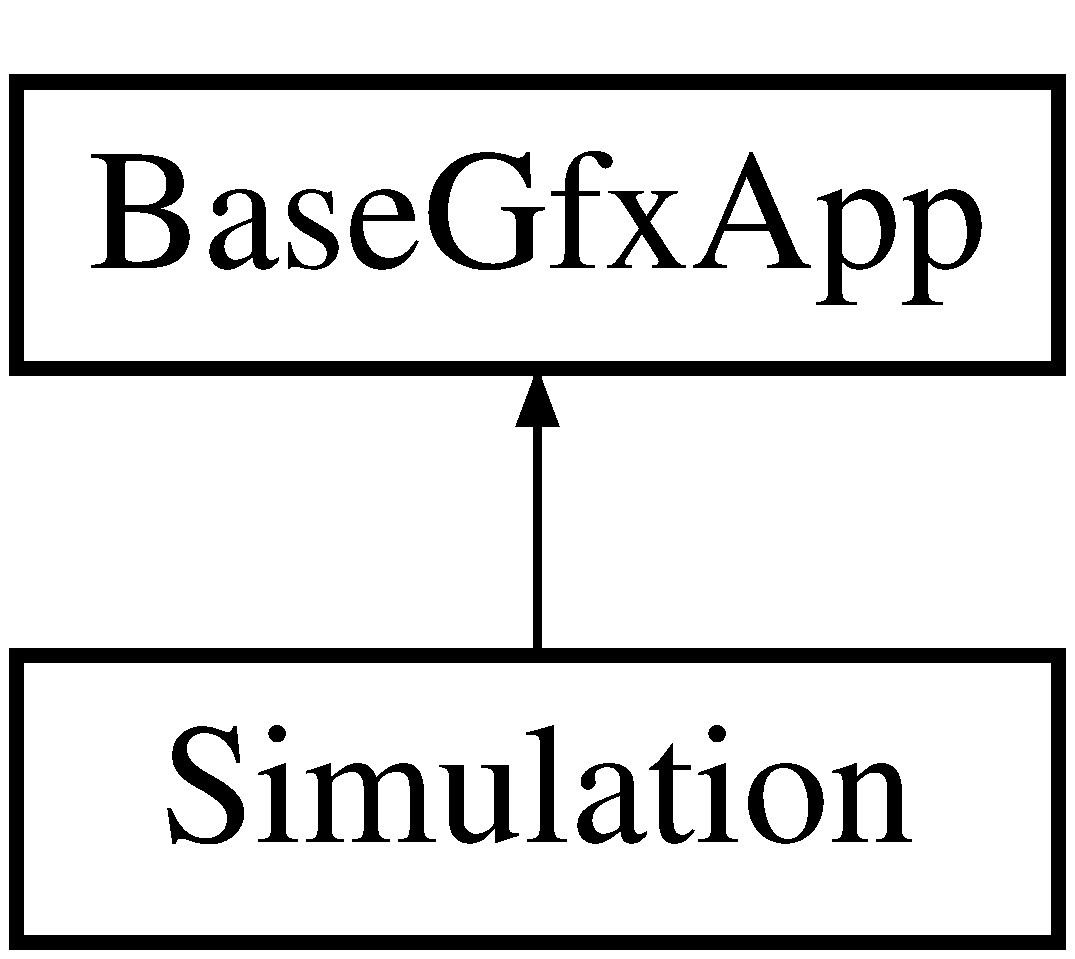
\includegraphics[height=2.000000cm]{classSimulation}
\end{center}
\end{figure}
\subsection*{Public Types}
\begin{DoxyCompactItemize}
\item 
enum \hyperlink{classSimulation_a0fd1c91d4e7699e893929d56b60a60bf}{U\-I\-Control\-Type} \{ {\bfseries U\-I\-\_\-\-Q\-U\-I\-T} = 0, 
{\bfseries U\-I\-\_\-\-S\-T\-A\-R\-T} = 1, 
{\bfseries U\-I\-\_\-\-P\-A\-U\-S\-E} = 2, 
{\bfseries U\-I\-\_\-\-R\-E\-S\-U\-M\-E} = 3
 \}
\begin{DoxyCompactList}\small\item\em enum the control type to setup button with four functions start,pause,resume and quit \end{DoxyCompactList}\end{DoxyCompactItemize}
\subsection*{Public Member Functions}
\begin{DoxyCompactItemize}
\item 
\hyperlink{classSimulation_a4c669ceaa34c7130966ce45f9de75fbe}{Simulation} (int argc, char $\ast$argv\mbox{[}$\,$\mbox{]}, int width, int height)
\begin{DoxyCompactList}\small\item\em initialize \hyperlink{classSimulation}{Simulation} class \end{DoxyCompactList}\item 
\hyperlink{classSimulation_a80fad3f57dfaf195a36f7bc49bc88279}{$\sim$\-Simulation} ()
\begin{DoxyCompactList}\small\item\em for the environment and Robot,Obstacle, Target object can have the setup for theris reder ans sence function and so on \end{DoxyCompactList}\item 
\hypertarget{classSimulation_ad50fa94a630141b3221d2d946a4bb11b}{void \hyperlink{classSimulation_ad50fa94a630141b3221d2d946a4bb11b}{glui\-Control} (int ctrl\-I\-D)}\label{classSimulation_ad50fa94a630141b3221d2d946a4bb11b}

\begin{DoxyCompactList}\small\item\em control with ctrl\-Id the control setup \end{DoxyCompactList}\item 
\hypertarget{classSimulation_a449dcb7d97dfba99efe770de2f399c31}{void \hyperlink{classSimulation_a449dcb7d97dfba99efe770de2f399c31}{display} ()}\label{classSimulation_a449dcb7d97dfba99efe770de2f399c31}

\begin{DoxyCompactList}\small\item\em display the environment call environment update to simulate anything \end{DoxyCompactList}\item 
\hypertarget{classSimulation_a786d1ba31d29937f0ac6f3ea88f8a607}{void {\bfseries left\-Mouse\-Down} (int x, int y)}\label{classSimulation_a786d1ba31d29937f0ac6f3ea88f8a607}

\item 
\hypertarget{classSimulation_a62ef254d85017074cd521a5787b5a234}{void {\bfseries left\-Mouse\-Up} (int x, int y)}\label{classSimulation_a62ef254d85017074cd521a5787b5a234}

\end{DoxyCompactItemize}
\subsection*{Static Public Member Functions}
\begin{DoxyCompactItemize}
\item 
static void \hyperlink{classSimulation_abaa3b54d7bf4b7cb263a9aa09bccfa2f}{Start} ()
\begin{DoxyCompactList}\small\item\em button's function \end{DoxyCompactList}\item 
\hypertarget{classSimulation_ac973ce238bc70e9be327f60c694b1b65}{static void {\bfseries Pause} ()}\label{classSimulation_ac973ce238bc70e9be327f60c694b1b65}

\item 
\hypertarget{classSimulation_a644cd9822aa95007143a108a7551780a}{static void {\bfseries Resume} ()}\label{classSimulation_a644cd9822aa95007143a108a7551780a}

\end{DoxyCompactItemize}
\subsection*{Protected Attributes}
\begin{DoxyCompactItemize}
\item 
\hypertarget{classSimulation_a033a987c62d4a02161444c1cb1e79d92}{\hyperlink{classEnvironmentClass}{Environment\-Class} \hyperlink{classSimulation_a033a987c62d4a02161444c1cb1e79d92}{environment}}\label{classSimulation_a033a987c62d4a02161444c1cb1e79d92}

\begin{DoxyCompactList}\small\item\em environment \end{DoxyCompactList}\end{DoxyCompactItemize}
\subsection*{Static Protected Attributes}
\begin{DoxyCompactItemize}
\item 
static bool \hyperlink{classSimulation_a738b72757500bc1c1fb33ffa42053c71}{Unmoved} = false
\begin{DoxyCompactList}\small\item\em variable setting up to judge the condition for the movement so that use it to control the button's function \end{DoxyCompactList}\end{DoxyCompactItemize}
\subsection*{Additional Inherited Members}


\subsection{Detailed Description}
The \hyperlink{classSimulation}{Simulation} class. This sets up the G\-U\-I and the drawing environment. 

\subsection{Member Enumeration Documentation}
\hypertarget{classSimulation_a0fd1c91d4e7699e893929d56b60a60bf}{\index{Simulation@{Simulation}!U\-I\-Control\-Type@{U\-I\-Control\-Type}}
\index{U\-I\-Control\-Type@{U\-I\-Control\-Type}!Simulation@{Simulation}}
\subsubsection[{U\-I\-Control\-Type}]{\setlength{\rightskip}{0pt plus 5cm}enum {\bf Simulation\-::\-U\-I\-Control\-Type}}}\label{classSimulation_a0fd1c91d4e7699e893929d56b60a60bf}


enum the control type to setup button with four functions start,pause,resume and quit 

\begin{DoxyAuthor}{Author}
Xinyue Zhang 
\end{DoxyAuthor}


\subsection{Constructor \& Destructor Documentation}
\hypertarget{classSimulation_a4c669ceaa34c7130966ce45f9de75fbe}{\index{Simulation@{Simulation}!Simulation@{Simulation}}
\index{Simulation@{Simulation}!Simulation@{Simulation}}
\subsubsection[{Simulation}]{\setlength{\rightskip}{0pt plus 5cm}Simulation\-::\-Simulation (
\begin{DoxyParamCaption}
\item[{int}]{argc, }
\item[{char $\ast$}]{argv\mbox{[}$\,$\mbox{]}, }
\item[{int}]{width, }
\item[{int}]{height}
\end{DoxyParamCaption}
)}}\label{classSimulation_a4c669ceaa34c7130966ce45f9de75fbe}


initialize \hyperlink{classSimulation}{Simulation} class 

initialize the \hyperlink{classSimulation}{Simulation} class inherited from \hyperlink{classBaseGfxApp}{Base\-Gfx\-App} creates a basic U\-I panel with quit button create buttons on the U\-I panel reperate the U\-I control type and the functions on each button \begin{DoxyAuthor}{Author}
Jiajun Ni, Xinyue Zhang
\end{DoxyAuthor}

\begin{DoxyCode}
 Initialize OpenGL
  /
glClearColor(0.0f, 0.0f, 0.0f, 1.0f);
glEnable(GL\_BLEND);
glBlendFunc(GL\_SRC\_ALPHA, GL\_ONE\_MINUS\_SRC\_ALPHA);
glMatrixMode(GL\_PROJECTION);
glLoadIdentity();
glMatrixMode(GL\_MODELVIEW);
glLoadIdentity();
gluOrtho2D(0, m\_width, 0, m\_height);
glViewport(0, 0, m\_width, m\_height);

\hyperlink{classEnvironmentClass_a3af1904397a45c74acbc0c8246c0317d}{EnvironmentClass::init}(width, height);
\end{DoxyCode}
\hypertarget{classSimulation_a80fad3f57dfaf195a36f7bc49bc88279}{\index{Simulation@{Simulation}!$\sim$\-Simulation@{$\sim$\-Simulation}}
\index{$\sim$\-Simulation@{$\sim$\-Simulation}!Simulation@{Simulation}}
\subsubsection[{$\sim$\-Simulation}]{\setlength{\rightskip}{0pt plus 5cm}Simulation\-::$\sim$\-Simulation (
\begin{DoxyParamCaption}
{}
\end{DoxyParamCaption}
)}}\label{classSimulation_a80fad3f57dfaf195a36f7bc49bc88279}


for the environment and Robot,Obstacle, Target object can have the setup for theris reder ans sence function and so on 

\begin{DoxyAuthor}{Author}
Jiajun Ni 
\end{DoxyAuthor}


\subsection{Member Function Documentation}
\hypertarget{classSimulation_abaa3b54d7bf4b7cb263a9aa09bccfa2f}{\index{Simulation@{Simulation}!Start@{Start}}
\index{Start@{Start}!Simulation@{Simulation}}
\subsubsection[{Start}]{\setlength{\rightskip}{0pt plus 5cm}void Simulation\-::\-Start (
\begin{DoxyParamCaption}
{}
\end{DoxyParamCaption}
)\hspace{0.3cm}{\ttfamily [static]}}}\label{classSimulation_abaa3b54d7bf4b7cb263a9aa09bccfa2f}


button's function 

the button function update unmoved conditions after clicking each button 

\subsection{Member Data Documentation}
\hypertarget{classSimulation_a738b72757500bc1c1fb33ffa42053c71}{\index{Simulation@{Simulation}!Unmoved@{Unmoved}}
\index{Unmoved@{Unmoved}!Simulation@{Simulation}}
\subsubsection[{Unmoved}]{\setlength{\rightskip}{0pt plus 5cm}bool Simulation\-::\-Unmoved = false\hspace{0.3cm}{\ttfamily [static]}, {\ttfamily [protected]}}}\label{classSimulation_a738b72757500bc1c1fb33ffa42053c71}


variable setting up to judge the condition for the movement so that use it to control the button's function 

initialize the Unmoved as all the objects in the screen has started moving 

The documentation for this class was generated from the following files\-:\begin{DoxyCompactItemize}
\item 
\hyperlink{Simulation_8h}{Simulation.\-h}\item 
\hyperlink{Simulation_8cpp}{Simulation.\-cpp}\end{DoxyCompactItemize}

\chapter{File Documentation}
\hypertarget{BaseGfxApp_8cpp}{\section{Base\-Gfx\-App.\-cpp File Reference}
\label{BaseGfxApp_8cpp}\index{Base\-Gfx\-App.\-cpp@{Base\-Gfx\-App.\-cpp}}
}


\hyperlink{classBaseGfxApp}{Base\-Gfx\-App}.  


{\ttfamily \#include \char`\"{}Base\-Gfx\-App.\-h\char`\"{}}\\*
\subsection*{Macros}
\begin{DoxyCompactItemize}
\item 
\hypertarget{BaseGfxApp_8cpp_a38533d3b08eadb4b2e6fe2f443dd83f1}{\#define {\bfseries I\-N\-I\-T\-\_\-\-W\-I\-D\-T\-H}~800}\label{BaseGfxApp_8cpp_a38533d3b08eadb4b2e6fe2f443dd83f1}

\item 
\hypertarget{BaseGfxApp_8cpp_acd7e35d0c6cca5b5b665b77b5377c4a0}{\#define {\bfseries I\-N\-I\-T\-\_\-\-H\-E\-I\-G\-H\-T}~600}\label{BaseGfxApp_8cpp_acd7e35d0c6cca5b5b665b77b5377c4a0}

\end{DoxyCompactItemize}


\subsection{Detailed Description}
\hyperlink{classBaseGfxApp}{Base\-Gfx\-App}. 
\hypertarget{BaseGfxApp_8h}{\section{Base\-Gfx\-App.\-h File Reference}
\label{BaseGfxApp_8h}\index{Base\-Gfx\-App.\-h@{Base\-Gfx\-App.\-h}}
}


\hyperlink{classBaseGfxApp}{Base\-Gfx\-App} header file.  


{\ttfamily \#include \char`\"{}Common.\-h\char`\"{}}\\*
\subsection*{Classes}
\begin{DoxyCompactItemize}
\item 
class \hyperlink{classBaseGfxApp}{Base\-Gfx\-App}
\begin{DoxyCompactList}\small\item\em based \hyperlink{classBaseGfxApp}{Base\-Gfx\-App} \end{DoxyCompactList}\end{DoxyCompactItemize}


\subsection{Detailed Description}
\hyperlink{classBaseGfxApp}{Base\-Gfx\-App} header file. 
\hypertarget{Common_8h}{\section{Common.\-h File Reference}
\label{Common_8h}\index{Common.\-h@{Common.\-h}}
}


obstacles (plane or circular obstacles), G\-Lpostion  


{\ttfamily \#include $<$iostream$>$}\\*
{\ttfamily \#include $<$string$>$}\\*
{\ttfamily \#include $<$memory$>$}\\*
{\ttfamily \#include $<$cassert$>$}\\*
{\ttfamily \#include $<$cmath$>$}\\*
{\ttfamily \#include $<$utility$>$}\\*
{\ttfamily \#include $<$G\-L/gl.\-h$>$}\\*
{\ttfamily \#include $<$G\-L/glui.\-h$>$}\\*
\subsection*{Classes}
\begin{DoxyCompactItemize}
\item 
struct \hyperlink{structGLPosition}{G\-L\-Position}
\begin{DoxyCompactList}\small\item\em get the G\-Lposition from the struct \end{DoxyCompactList}\item 
class \hyperlink{classObject}{Object}
\begin{DoxyCompactList}\small\item\em base object class obstacle, robot, and any other simulate object. \end{DoxyCompactList}\end{DoxyCompactItemize}
\subsection*{Macros}
\begin{DoxyCompactItemize}
\item 
\hypertarget{Common_8h_a598a3330b3c21701223ee0ca14316eca}{\#define {\bfseries P\-I}~3.\-14159265}\label{Common_8h_a598a3330b3c21701223ee0ca14316eca}

\end{DoxyCompactItemize}
\subsection*{Typedefs}
\begin{DoxyCompactItemize}
\item 
typedef struct \hyperlink{structGLPosition}{G\-L\-Position} \hyperlink{Common_8h_a5113b6588451c418d38d8b3681eb6040}{gl\-Color\-Vec}
\begin{DoxyCompactList}\small\item\em get the G\-Lposition from the struct \end{DoxyCompactList}\end{DoxyCompactItemize}


\subsection{Detailed Description}
obstacles (plane or circular obstacles), G\-Lpostion \begin{DoxyAuthor}{Author}
Jiajun Ni 
\end{DoxyAuthor}


\subsection{Typedef Documentation}
\hypertarget{Common_8h_a5113b6588451c418d38d8b3681eb6040}{\index{Common.\-h@{Common.\-h}!gl\-Color\-Vec@{gl\-Color\-Vec}}
\index{gl\-Color\-Vec@{gl\-Color\-Vec}!Common.h@{Common.\-h}}
\subsubsection[{gl\-Color\-Vec}]{\setlength{\rightskip}{0pt plus 5cm}typedef struct {\bf G\-L\-Position}  {\bf gl\-Color\-Vec}}}\label{Common_8h_a5113b6588451c418d38d8b3681eb6040}


get the G\-Lposition from the struct 

\begin{DoxyAuthor}{Author}
Jiajun Ni 
\end{DoxyAuthor}

\hypertarget{CommonTest_8h}{\section{Common\-Test.\-h File Reference}
\label{CommonTest_8h}\index{Common\-Test.\-h@{Common\-Test.\-h}}
}


test the position, orientation, speed, detect\-Wall, detect\-Obstacles, detect\-Target  


{\ttfamily \#include $<$cxxtest/\-Test\-Suite.\-h$>$}\\*
{\ttfamily \#include \char`\"{}Common.\-h\char`\"{}}\\*
{\ttfamily \#include \char`\"{}Obstacle.\-h\char`\"{}}\\*
{\ttfamily \#include \char`\"{}Simulation.\-h\char`\"{}}\\*
\subsection*{Classes}
\begin{DoxyCompactItemize}
\item 
class \hyperlink{classCommonTests}{Common\-Tests}
\begin{DoxyCompactList}\small\item\em test function for G\-Lposition struct, object overlapping and detect\-Wall \end{DoxyCompactList}\end{DoxyCompactItemize}


\subsection{Detailed Description}
test the position, orientation, speed, detect\-Wall, detect\-Obstacles, detect\-Target \begin{DoxyAuthor}{Author}
Jiajun Ni 
\end{DoxyAuthor}

\hypertarget{EnvironmentClass_8h}{\section{Environment\-Class.\-h File Reference}
\label{EnvironmentClass_8h}\index{Environment\-Class.\-h@{Environment\-Class.\-h}}
}


Class to contain physical objects, sizes/position of all objects and contains info on where the borders are in the window.  


{\ttfamily \#include \char`\"{}Common.\-h\char`\"{}}\\*
{\ttfamily \#include \char`\"{}Obstacle.\-h\char`\"{}}\\*
{\ttfamily \#include \char`\"{}Robot\-Class.\-h\char`\"{}}\\*
\subsection*{Classes}
\begin{DoxyCompactItemize}
\item 
class \hyperlink{classEnvironmentClass}{Environment\-Class}
\begin{DoxyCompactList}\small\item\em Class to contain physical objects, sizes/position of all objects and contains info on where the borders are in the window. \end{DoxyCompactList}\end{DoxyCompactItemize}


\subsection{Detailed Description}
Class to contain physical objects, sizes/position of all objects and contains info on where the borders are in the window. \begin{DoxyAuthor}{Author}
Jiajun Ni 
\end{DoxyAuthor}

\hypertarget{EnvironmentClassTest_8h}{\section{Environment\-Class\-Test.\-h File Reference}
\label{EnvironmentClassTest_8h}\index{Environment\-Class\-Test.\-h@{Environment\-Class\-Test.\-h}}
}


environment test for sensor,random position, distance  


{\ttfamily \#include $<$cxxtest/\-Test\-Suite.\-h$>$}\\*
{\ttfamily \#include \char`\"{}Environment\-Class.\-h\char`\"{}}\\*
{\ttfamily \#include \char`\"{}Simulation.\-h\char`\"{}}\\*
\subsection*{Classes}
\begin{DoxyCompactItemize}
\item 
class \hyperlink{classEnvironmentClassTests}{Environment\-Class\-Tests}
\begin{DoxyCompactList}\small\item\em environment test for sensor,random position, distance \end{DoxyCompactList}\end{DoxyCompactItemize}


\subsection{Detailed Description}
environment test for sensor,random position, distance \begin{DoxyAuthor}{Author}
Jiajun Ni 
\end{DoxyAuthor}

\hypertarget{Obstacle_8h}{\section{Obstacle.\-h File Reference}
\label{Obstacle_8h}\index{Obstacle.\-h@{Obstacle.\-h}}
}


draw obstacles avoid overlapping the robot  


{\ttfamily \#include \char`\"{}Common.\-h\char`\"{}}\\*
\subsection*{Classes}
\begin{DoxyCompactItemize}
\item 
class \hyperlink{classCircularObstacle}{Circular\-Obstacle}
\begin{DoxyCompactList}\small\item\em obstacle with circul \end{DoxyCompactList}\end{DoxyCompactItemize}


\subsection{Detailed Description}
draw obstacles avoid overlapping the robot \begin{DoxyAuthor}{Author}
Jiajun Ni 
\end{DoxyAuthor}

\hypertarget{ObstacleTest_8h}{\section{Obstacle\-Test.\-h File Reference}
\label{ObstacleTest_8h}\index{Obstacle\-Test.\-h@{Obstacle\-Test.\-h}}
}


test the position, orientation, speed, detect\-Wall, detect\-Obstacles, detect\-Target  


{\ttfamily \#include $<$cxxtest/\-Test\-Suite.\-h$>$}\\*
{\ttfamily \#include \char`\"{}Obstacle.\-h\char`\"{}}\\*
{\ttfamily \#include \char`\"{}Simulation.\-h\char`\"{}}\\*
\subsection*{Classes}
\begin{DoxyCompactItemize}
\item 
class \hyperlink{classObstacleTests}{Obstacle\-Tests}
\begin{DoxyCompactList}\small\item\em test for the obstacle's basic attributes \end{DoxyCompactList}\end{DoxyCompactItemize}


\subsection{Detailed Description}
test the position, orientation, speed, detect\-Wall, detect\-Obstacles, detect\-Target \begin{DoxyAuthor}{Author}
Jiajun Ni 
\end{DoxyAuthor}

\hypertarget{RobotClass_8cpp}{\section{Robot\-Class.\-cpp File Reference}
\label{RobotClass_8cpp}\index{Robot\-Class.\-cpp@{Robot\-Class.\-cpp}}
}


detect\-Wall, detet\-Obstacles, detect\-Target ,draw robot with a line  


{\ttfamily \#include \char`\"{}Robot\-Class.\-h\char`\"{}}\\*


\subsection{Detailed Description}
detect\-Wall, detet\-Obstacles, detect\-Target ,draw robot with a line \begin{DoxyAuthor}{Author}
Jiajun Ni` 
\end{DoxyAuthor}

\hypertarget{RobotClass_8h}{\section{Robot\-Class.\-h File Reference}
\label{RobotClass_8h}\index{Robot\-Class.\-h@{Robot\-Class.\-h}}
}


header of \hyperlink{classRobotClass}{Robot\-Class}  


{\ttfamily \#include \char`\"{}Common.\-h\char`\"{}}\\*
\subsection*{Classes}
\begin{DoxyCompactItemize}
\item 
class \hyperlink{classRobotClass}{Robot\-Class}
\begin{DoxyCompactList}\small\item\em \hyperlink{classRobotClass}{Robot\-Class}. This provides means to store and alter robot state. \end{DoxyCompactList}\end{DoxyCompactItemize}


\subsection{Detailed Description}
header of \hyperlink{classRobotClass}{Robot\-Class} 
\hypertarget{RobotTests_8h}{\section{Robot\-Tests.\-h File Reference}
\label{RobotTests_8h}\index{Robot\-Tests.\-h@{Robot\-Tests.\-h}}
}


test the position, orientation, speed, detect\-Wall, detect\-Obstacles, detect\-Target  


{\ttfamily \#include $<$cxxtest/\-Test\-Suite.\-h$>$}\\*
{\ttfamily \#include \char`\"{}Robot\-Class.\-h\char`\"{}}\\*
{\ttfamily \#include \char`\"{}Simulation.\-h\char`\"{}}\\*
\subsection*{Classes}
\begin{DoxyCompactItemize}
\item 
class \hyperlink{classRobotTests}{Robot\-Tests}
\begin{DoxyCompactList}\small\item\em Test robot's position,orientation, speed, movement and the detection of obstacle. \end{DoxyCompactList}\end{DoxyCompactItemize}


\subsection{Detailed Description}
test the position, orientation, speed, detect\-Wall, detect\-Obstacles, detect\-Target 
\hypertarget{Simulation_8cpp}{\section{Simulation.\-cpp File Reference}
\label{Simulation_8cpp}\index{Simulation.\-cpp@{Simulation.\-cpp}}
}


generate basic simulated control  


{\ttfamily \#include \char`\"{}Simulation.\-h\char`\"{}}\\*


\subsection{Detailed Description}
generate basic simulated control \begin{DoxyAuthor}{Author}
Jiajun Ni 
\end{DoxyAuthor}

\hypertarget{Simulation_8h}{\section{Simulation.\-h File Reference}
\label{Simulation_8h}\index{Simulation.\-h@{Simulation.\-h}}
}


generate baisc simulated control  


{\ttfamily \#include \char`\"{}Base\-Gfx\-App.\-h\char`\"{}}\\*
{\ttfamily \#include \char`\"{}Environment\-Class.\-h\char`\"{}}\\*
{\ttfamily \#include \char`\"{}Common.\-h\char`\"{}}\\*
\subsection*{Classes}
\begin{DoxyCompactItemize}
\item 
class \hyperlink{classSimulation}{Simulation}
\begin{DoxyCompactList}\small\item\em The \hyperlink{classSimulation}{Simulation} class. This sets up the G\-U\-I and the drawing environment. \end{DoxyCompactList}\end{DoxyCompactItemize}


\subsection{Detailed Description}
generate baisc simulated control \begin{DoxyAuthor}{Author}
Jiajun Ni 
\end{DoxyAuthor}

%--- End generated contents ---

% Index
\newpage
\phantomsection
\addcontentsline{toc}{chapter}{Index}
\printindex

\end{document}
